% Created by tikzDevice version 0.12.3 on 2021-01-31 17:57:48
% !TEX encoding = UTF-8 Unicode
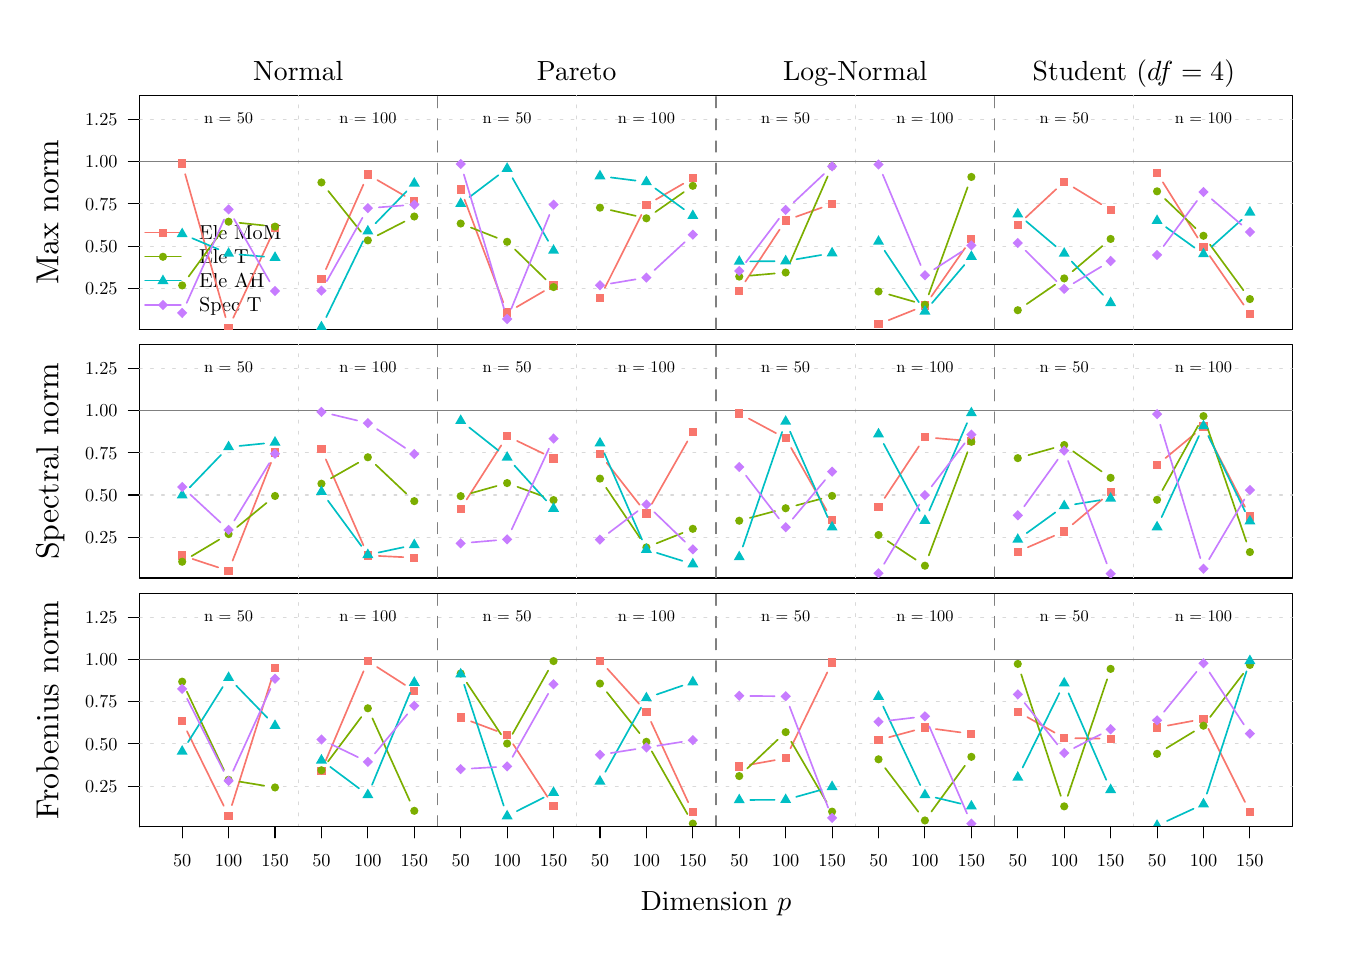
\begin{tikzpicture}[x=1pt,y=1pt]
\definecolor{fillColor}{RGB}{255,255,255}
\path[use as bounding box,fill=fillColor,fill opacity=0.00] (0,0) rectangle (469.75,325.21);
\begin{scope}
\path[clip] (  0.00,  0.00) rectangle (469.75,325.21);
\definecolor{drawColor}{RGB}{0,0,0}

\path[draw=drawColor,line width= 0.4pt,line join=round,line cap=round] ( 40.39,216.28) --
	(457.08,216.28) --
	(457.08,300.66) --
	( 40.39,300.66) --
	( 40.39,216.28);

\path[draw=drawColor,line width= 0.4pt,line join=round,line cap=round] ( 40.39,231.00) -- ( 40.39,292.04);

\path[draw=drawColor,line width= 0.4pt,line join=round,line cap=round] ( 40.39,231.00) -- ( 36.43,231.00);

\path[draw=drawColor,line width= 0.4pt,line join=round,line cap=round] ( 40.39,246.26) -- ( 36.43,246.26);

\path[draw=drawColor,line width= 0.4pt,line join=round,line cap=round] ( 40.39,261.52) -- ( 36.43,261.52);

\path[draw=drawColor,line width= 0.4pt,line join=round,line cap=round] ( 40.39,276.78) -- ( 36.43,276.78);

\path[draw=drawColor,line width= 0.4pt,line join=round,line cap=round] ( 40.39,292.04) -- ( 36.43,292.04);

\node[text=drawColor,anchor=base east,inner sep=0pt, outer sep=0pt, scale=  0.66] at ( 32.47,228.73) {0.25};

\node[text=drawColor,anchor=base east,inner sep=0pt, outer sep=0pt, scale=  0.66] at ( 32.47,243.99) {0.50};

\node[text=drawColor,anchor=base east,inner sep=0pt, outer sep=0pt, scale=  0.66] at ( 32.47,259.25) {0.75};

\node[text=drawColor,anchor=base east,inner sep=0pt, outer sep=0pt, scale=  0.66] at ( 32.47,274.51) {1.00};

\node[text=drawColor,anchor=base east,inner sep=0pt, outer sep=0pt, scale=  0.66] at ( 32.47,289.77) {1.25};
\end{scope}
\begin{scope}
\path[clip] ( 40.39,216.28) rectangle (457.08,300.66);
\definecolor{drawColor}{gray}{0.85}

\path[draw=drawColor,line width= 0.4pt,dash pattern=on 1pt off 3pt ,line join=round,line cap=round] ( 40.39,231.00) -- (457.08,231.00);

\path[draw=drawColor,line width= 0.4pt,dash pattern=on 1pt off 3pt ,line join=round,line cap=round] ( 40.39,246.26) -- (457.08,246.26);

\path[draw=drawColor,line width= 0.4pt,dash pattern=on 1pt off 3pt ,line join=round,line cap=round] ( 40.39,261.52) -- (457.08,261.52);

\path[draw=drawColor,line width= 0.4pt,dash pattern=on 1pt off 3pt ,line join=round,line cap=round] ( 40.39,276.78) -- (457.08,276.78);

\path[draw=drawColor,line width= 0.4pt,dash pattern=on 1pt off 3pt ,line join=round,line cap=round] ( 40.39,292.04) -- (457.08,292.04);

\path[draw=drawColor,line width= 0.4pt,dash pattern=on 1pt off 3pt ,line join=round,line cap=round] ( 97.76,216.28) -- ( 97.76,300.66);

\path[draw=drawColor,line width= 0.4pt,dash pattern=on 1pt off 3pt ,line join=round,line cap=round] (198.41,216.28) -- (198.41,300.66);

\path[draw=drawColor,line width= 0.4pt,dash pattern=on 1pt off 3pt ,line join=round,line cap=round] (299.06,216.28) -- (299.06,300.66);

\path[draw=drawColor,line width= 0.4pt,dash pattern=on 1pt off 3pt ,line join=round,line cap=round] (399.71,216.28) -- (399.71,300.66);
\definecolor{drawColor}{gray}{0.50}

\path[draw=drawColor,line width= 0.4pt,dash pattern=on 4pt off 4pt ,line join=round,line cap=round] (148.09,216.28) -- (148.09,300.66);

\path[draw=drawColor,line width= 0.4pt,dash pattern=on 4pt off 4pt ,line join=round,line cap=round] (248.74,216.28) -- (248.74,300.66);

\path[draw=drawColor,line width= 0.4pt,dash pattern=on 4pt off 4pt ,line join=round,line cap=round] (349.39,216.28) -- (349.39,300.66);
\end{scope}
\begin{scope}
\path[clip] (  0.00,  0.00) rectangle (469.75,325.21);
\definecolor{drawColor}{RGB}{0,0,0}

\node[text=drawColor,rotate= 90.00,anchor=base,inner sep=0pt, outer sep=0pt, scale=  1.15] at ( 11.09,258.47) {Max norm};
\end{scope}
\begin{scope}
\path[clip] ( 40.39,216.28) rectangle (457.08,300.66);
\definecolor{drawColor}{gray}{0.50}

\path[draw=drawColor,line width= 0.4pt,line join=round,line cap=round] ( 40.39,276.78) -- (457.08,276.78);
\end{scope}
\begin{scope}
\path[clip] (  0.00,  0.00) rectangle (469.75,325.21);
\definecolor{drawColor}{RGB}{0,0,0}

\node[text=drawColor,anchor=base,inner sep=0pt, outer sep=0pt, scale=  1.00] at ( 97.76,306.21) {Normal};

\node[text=drawColor,anchor=base,inner sep=0pt, outer sep=0pt, scale=  1.00] at (198.41,306.21) {Pareto};

\node[text=drawColor,anchor=base,inner sep=0pt, outer sep=0pt, scale=  1.00] at (299.06,306.21) {Log-Normal};

\node[text=drawColor,anchor=base,inner sep=0pt, outer sep=0pt, scale=  1.00] at (399.71,306.21) {Student ($df = 4$)};
\end{scope}
\begin{scope}
\path[clip] ( 40.39,216.28) rectangle (457.08,300.66);
\definecolor{drawColor}{RGB}{0,0,0}

\node[text=drawColor,anchor=base,inner sep=0pt, outer sep=0pt, scale=  0.59] at ( 72.60,290.43) {n = 50};

\node[text=drawColor,anchor=base,inner sep=0pt, outer sep=0pt, scale=  0.59] at (122.92,290.43) {n = 100};

\node[text=drawColor,anchor=base,inner sep=0pt, outer sep=0pt, scale=  0.59] at (173.25,290.43) {n = 50};

\node[text=drawColor,anchor=base,inner sep=0pt, outer sep=0pt, scale=  0.59] at (223.57,290.43) {n = 100};

\node[text=drawColor,anchor=base,inner sep=0pt, outer sep=0pt, scale=  0.59] at (273.90,290.43) {n = 50};

\node[text=drawColor,anchor=base,inner sep=0pt, outer sep=0pt, scale=  0.59] at (324.22,290.43) {n = 100};

\node[text=drawColor,anchor=base,inner sep=0pt, outer sep=0pt, scale=  0.59] at (374.55,290.43) {n = 50};

\node[text=drawColor,anchor=base,inner sep=0pt, outer sep=0pt, scale=  0.59] at (424.87,290.43) {n = 100};
\definecolor{drawColor}{RGB}{248,118,109}

\path[draw=drawColor,line width= 0.4pt,line join=round,line cap=round] ( 42.35,251.13) -- ( 55.42,251.13);
\definecolor{drawColor}{RGB}{124,174,0}

\path[draw=drawColor,line width= 0.4pt,line join=round,line cap=round] ( 42.35,242.42) -- ( 55.42,242.42);
\definecolor{drawColor}{RGB}{0,191,196}

\path[draw=drawColor,line width= 0.4pt,line join=round,line cap=round] ( 42.35,233.71) -- ( 55.42,233.71);
\definecolor{drawColor}{RGB}{199,124,255}

\path[draw=drawColor,line width= 0.4pt,line join=round,line cap=round] ( 42.35,224.99) -- ( 55.42,224.99);
\definecolor{fillColor}{RGB}{248,118,109}

\path[fill=fillColor] ( 47.40,249.64) --
	( 50.37,249.64) --
	( 50.37,252.61) --
	( 47.40,252.61) --
	cycle;
\definecolor{fillColor}{RGB}{124,174,0}

\path[fill=fillColor] ( 48.89,242.42) circle (  1.48);
\definecolor{fillColor}{RGB}{0,191,196}

\path[fill=fillColor] ( 48.89,236.02) --
	( 50.89,232.55) --
	( 46.89,232.55) --
	cycle;
\definecolor{fillColor}{RGB}{199,124,255}

\path[fill=fillColor] ( 47.03,224.99) --
	( 48.89,226.85) --
	( 50.74,224.99) --
	( 48.89,223.14) --
	cycle;
\definecolor{drawColor}{RGB}{0,0,0}

\node[text=drawColor,anchor=base west,inner sep=0pt, outer sep=0pt, scale=  0.73] at ( 61.95,248.63) {Ele MoM};

\node[text=drawColor,anchor=base west,inner sep=0pt, outer sep=0pt, scale=  0.73] at ( 61.95,239.92) {Ele T};

\node[text=drawColor,anchor=base west,inner sep=0pt, outer sep=0pt, scale=  0.73] at ( 61.95,231.21) {Ele AH};

\node[text=drawColor,anchor=base west,inner sep=0pt, outer sep=0pt, scale=  0.73] at ( 61.95,222.49) {Spec T};
\definecolor{drawColor}{RGB}{248,118,109}

\path[draw=drawColor,line width= 0.6pt,line join=round,line cap=round] ( 56.90,272.31) -- ( 71.52,220.56);

\path[draw=drawColor,line width= 0.6pt,line join=round,line cap=round] ( 74.27,220.34) -- ( 87.70,249.16);
\definecolor{fillColor}{RGB}{248,118,109}

\path[fill=fillColor] ( 54.34,274.64) --
	( 57.31,274.64) --
	( 57.31,277.61) --
	( 54.34,277.61) --
	cycle;

\path[fill=fillColor] ( 71.11,215.27) --
	( 74.08,215.27) --
	( 74.08,218.24) --
	( 71.11,218.24) --
	cycle;

\path[fill=fillColor] ( 87.89,251.27) --
	( 90.86,251.27) --
	( 90.86,254.24) --
	( 87.89,254.24) --
	cycle;
\definecolor{drawColor}{RGB}{124,174,0}

\path[draw=drawColor,line width= 0.6pt,line join=round,line cap=round] ( 58.16,235.27) -- ( 70.27,251.90);

\path[draw=drawColor,line width= 0.6pt,line join=round,line cap=round] ( 76.54,254.68) -- ( 85.44,253.74);
\definecolor{fillColor}{RGB}{124,174,0}

\path[fill=fillColor] ( 55.83,232.07) circle (  1.48);

\path[fill=fillColor] ( 72.60,255.10) circle (  1.48);

\path[fill=fillColor] ( 89.38,253.32) circle (  1.48);
\definecolor{drawColor}{RGB}{0,191,196}

\path[draw=drawColor,line width= 0.6pt,line join=round,line cap=round] ( 59.47,249.12) -- ( 68.95,245.12);

\path[draw=drawColor,line width= 0.6pt,line join=round,line cap=round] ( 76.55,243.24) -- ( 85.43,242.46);
\definecolor{fillColor}{RGB}{0,191,196}

\path[fill=fillColor] ( 55.83,252.97) --
	( 57.82,249.51) --
	( 53.83,249.51) --
	cycle;

\path[fill=fillColor] ( 72.60,245.89) --
	( 74.60,242.43) --
	( 70.60,242.43) --
	cycle;

\path[fill=fillColor] ( 89.38,244.43) --
	( 91.37,240.97) --
	( 87.38,240.97) --
	cycle;
\definecolor{drawColor}{RGB}{199,124,255}

\path[draw=drawColor,line width= 0.6pt,line join=round,line cap=round] ( 57.45,225.74) -- ( 70.98,255.91);

\path[draw=drawColor,line width= 0.6pt,line join=round,line cap=round] ( 74.56,256.08) -- ( 87.42,233.49);
\definecolor{fillColor}{RGB}{199,124,255}

\path[fill=fillColor] ( 53.97,222.13) --
	( 55.83,223.99) --
	( 57.68,222.13) --
	( 55.83,220.27) --
	cycle;

\path[fill=fillColor] ( 70.74,259.52) --
	( 72.60,261.38) --
	( 74.46,259.52) --
	( 72.60,257.67) --
	cycle;

\path[fill=fillColor] ( 87.52,230.04) --
	( 89.38,231.90) --
	( 91.23,230.04) --
	( 89.38,228.19) --
	cycle;
\definecolor{drawColor}{RGB}{248,118,109}

\path[draw=drawColor,line width= 0.6pt,line join=round,line cap=round] (107.76,237.91) -- (121.32,268.50);

\path[draw=drawColor,line width= 0.6pt,line join=round,line cap=round] (126.35,270.14) -- (136.27,264.40);
\definecolor{fillColor}{RGB}{248,118,109}

\path[fill=fillColor] (104.66,232.81) --
	(107.63,232.81) --
	(107.63,235.78) --
	(104.66,235.78) --
	cycle;

\path[fill=fillColor] (121.44,270.64) --
	(124.41,270.64) --
	(124.41,273.61) --
	(121.44,273.61) --
	cycle;

\path[fill=fillColor] (138.21,260.93) --
	(141.19,260.93) --
	(141.19,263.90) --
	(138.21,263.90) --
	cycle;
\definecolor{drawColor}{RGB}{124,174,0}

\path[draw=drawColor,line width= 0.6pt,line join=round,line cap=round] (108.63,266.19) -- (120.45,251.44);

\path[draw=drawColor,line width= 0.6pt,line join=round,line cap=round] (126.45,250.16) -- (136.18,255.16);
\definecolor{fillColor}{RGB}{124,174,0}

\path[fill=fillColor] (106.15,269.28) circle (  1.48);

\path[fill=fillColor] (122.92,248.34) circle (  1.48);

\path[fill=fillColor] (139.70,256.97) circle (  1.48);
\definecolor{drawColor}{RGB}{0,191,196}

\path[draw=drawColor,line width= 0.6pt,line join=round,line cap=round] (107.88,220.58) -- (121.20,248.08);

\path[draw=drawColor,line width= 0.6pt,line join=round,line cap=round] (125.68,254.49) -- (136.94,266.09);
\definecolor{fillColor}{RGB}{0,191,196}

\path[fill=fillColor] (106.15,219.33) --
	(108.15,215.86) --
	(104.15,215.86) --
	cycle;

\path[fill=fillColor] (122.92,253.95) --
	(124.92,250.49) --
	(120.93,250.49) --
	cycle;

\path[fill=fillColor] (139.70,271.24) --
	(141.70,267.78) --
	(137.70,267.78) --
	cycle;
\definecolor{drawColor}{RGB}{199,124,255}

\path[draw=drawColor,line width= 0.6pt,line join=round,line cap=round] (108.09,233.63) -- (120.98,256.52);

\path[draw=drawColor,line width= 0.6pt,line join=round,line cap=round] (126.87,260.28) -- (135.75,260.96);
\definecolor{fillColor}{RGB}{199,124,255}

\path[fill=fillColor] (104.29,230.17) --
	(106.15,232.03) --
	(108.01,230.17) --
	(106.15,228.32) --
	cycle;

\path[fill=fillColor] (121.07,259.97) --
	(122.92,261.83) --
	(124.78,259.97) --
	(122.92,258.12) --
	cycle;

\path[fill=fillColor] (137.84,261.26) --
	(139.70,263.12) --
	(141.56,261.26) --
	(139.70,259.41) --
	cycle;
\definecolor{drawColor}{RGB}{248,118,109}

\path[draw=drawColor,line width= 0.6pt,line join=round,line cap=round] (157.87,263.06) -- (171.85,225.95);

\path[draw=drawColor,line width= 0.6pt,line join=round,line cap=round] (176.67,224.24) -- (186.60,230.03);
\definecolor{fillColor}{RGB}{248,118,109}

\path[fill=fillColor] (154.99,265.28) --
	(157.96,265.28) --
	(157.96,268.25) --
	(154.99,268.25) --
	cycle;

\path[fill=fillColor] (171.76,220.76) --
	(174.73,220.76) --
	(174.73,223.73) --
	(171.76,223.73) --
	cycle;

\path[fill=fillColor] (188.54,230.53) --
	(191.51,230.53) --
	(191.51,233.50) --
	(188.54,233.50) --
	cycle;
\definecolor{drawColor}{RGB}{124,174,0}

\path[draw=drawColor,line width= 0.6pt,line join=round,line cap=round] (160.16,252.98) -- (169.56,249.28);

\path[draw=drawColor,line width= 0.6pt,line join=round,line cap=round] (176.09,245.06) -- (187.19,234.24);
\definecolor{fillColor}{RGB}{124,174,0}

\path[fill=fillColor] (156.47,254.43) circle (  1.48);

\path[fill=fillColor] (173.25,247.83) circle (  1.48);

\path[fill=fillColor] (190.02,231.47) circle (  1.48);
\definecolor{drawColor}{RGB}{0,191,196}

\path[draw=drawColor,line width= 0.6pt,line join=round,line cap=round] (159.63,263.98) -- (170.09,271.90);

\path[draw=drawColor,line width= 0.6pt,line join=round,line cap=round] (175.20,270.85) -- (188.07,248.13);
\definecolor{fillColor}{RGB}{0,191,196}

\path[fill=fillColor] (156.47,263.90) --
	(158.47,260.44) --
	(154.48,260.44) --
	cycle;

\path[fill=fillColor] (173.25,276.60) --
	(175.25,273.14) --
	(171.25,273.14) --
	cycle;

\path[fill=fillColor] (190.02,246.99) --
	(192.02,243.53) --
	(188.03,243.53) --
	cycle;
\definecolor{drawColor}{RGB}{199,124,255}

\path[draw=drawColor,line width= 0.6pt,line join=round,line cap=round] (157.61,272.17) -- (172.11,223.73);

\path[draw=drawColor,line width= 0.6pt,line join=round,line cap=round] (174.74,223.61) -- (188.54,257.58);
\definecolor{fillColor}{RGB}{199,124,255}

\path[fill=fillColor] (154.62,275.96) --
	(156.47,277.82) --
	(158.33,275.96) --
	(156.47,274.10) --
	cycle;

\path[fill=fillColor] (171.39,219.94) --
	(173.25,221.79) --
	(175.11,219.94) --
	(173.25,218.08) --
	cycle;

\path[fill=fillColor] (188.17,261.25) --
	(190.02,263.11) --
	(191.88,261.25) --
	(190.02,259.40) --
	cycle;
\definecolor{drawColor}{RGB}{248,118,109}

\path[draw=drawColor,line width= 0.6pt,line join=round,line cap=round] (208.57,231.20) -- (221.80,257.58);

\path[draw=drawColor,line width= 0.6pt,line join=round,line cap=round] (227.00,263.10) -- (236.92,268.84);
\definecolor{fillColor}{RGB}{248,118,109}

\path[fill=fillColor] (205.31,226.17) --
	(208.28,226.17) --
	(208.28,229.14) --
	(205.31,229.14) --
	cycle;

\path[fill=fillColor] (222.09,259.63) --
	(225.06,259.63) --
	(225.06,262.60) --
	(222.09,262.60) --
	cycle;

\path[fill=fillColor] (238.86,269.33) --
	(241.83,269.33) --
	(241.83,272.30) --
	(238.86,272.30) --
	cycle;
\definecolor{drawColor}{RGB}{124,174,0}

\path[draw=drawColor,line width= 0.6pt,line join=round,line cap=round] (210.66,259.28) -- (219.72,257.20);

\path[draw=drawColor,line width= 0.6pt,line join=round,line cap=round] (226.82,258.59) -- (237.11,265.79);
\definecolor{fillColor}{RGB}{124,174,0}

\path[fill=fillColor] (206.80,260.17) circle (  1.48);

\path[fill=fillColor] (223.57,256.32) circle (  1.48);

\path[fill=fillColor] (240.35,268.06) circle (  1.48);
\definecolor{drawColor}{RGB}{0,191,196}

\path[draw=drawColor,line width= 0.6pt,line join=round,line cap=round] (210.73,271.08) -- (219.65,269.95);

\path[draw=drawColor,line width= 0.6pt,line join=round,line cap=round] (226.78,267.12) -- (237.15,259.57);
\definecolor{fillColor}{RGB}{0,191,196}

\path[fill=fillColor] (206.80,273.89) --
	(208.80,270.42) --
	(204.80,270.42) --
	cycle;

\path[fill=fillColor] (223.57,271.76) --
	(225.57,268.29) --
	(221.58,268.29) --
	cycle;

\path[fill=fillColor] (240.35,259.55) --
	(242.35,256.08) --
	(238.35,256.08) --
	cycle;
\definecolor{drawColor}{RGB}{199,124,255}

\path[draw=drawColor,line width= 0.6pt,line join=round,line cap=round] (210.71,232.76) -- (219.67,234.26);

\path[draw=drawColor,line width= 0.6pt,line join=round,line cap=round] (226.48,237.60) -- (237.44,247.72);
\definecolor{fillColor}{RGB}{199,124,255}

\path[fill=fillColor] (204.94,232.11) --
	(206.80,233.97) --
	(208.66,232.11) --
	(206.80,230.26) --
	cycle;

\path[fill=fillColor] (221.72,234.91) --
	(223.57,236.77) --
	(225.43,234.91) --
	(223.57,233.05) --
	cycle;

\path[fill=fillColor] (238.49,250.40) --
	(240.35,252.26) --
	(242.21,250.40) --
	(240.35,248.55) --
	cycle;
\definecolor{drawColor}{RGB}{248,118,109}

\path[draw=drawColor,line width= 0.6pt,line join=round,line cap=round] (259.31,233.48) -- (271.72,252.25);

\path[draw=drawColor,line width= 0.6pt,line join=round,line cap=round] (277.63,256.88) -- (286.94,260.19);
\definecolor{fillColor}{RGB}{248,118,109}

\path[fill=fillColor] (255.64,228.70) --
	(258.61,228.70) --
	(258.61,231.67) --
	(255.64,231.67) --
	cycle;

\path[fill=fillColor] (272.41,254.07) --
	(275.38,254.07) --
	(275.38,257.04) --
	(272.41,257.04) --
	cycle;

\path[fill=fillColor] (289.19,260.03) --
	(292.16,260.03) --
	(292.16,263.00) --
	(289.19,263.00) --
	cycle;
\definecolor{drawColor}{RGB}{124,174,0}

\path[draw=drawColor,line width= 0.6pt,line join=round,line cap=round] (261.07,235.61) -- (269.96,236.39);

\path[draw=drawColor,line width= 0.6pt,line join=round,line cap=round] (275.49,240.36) -- (289.09,271.49);
\definecolor{fillColor}{RGB}{124,174,0}

\path[fill=fillColor] (257.12,235.26) circle (  1.48);

\path[fill=fillColor] (273.90,236.73) circle (  1.48);

\path[fill=fillColor] (290.67,275.12) circle (  1.48);
\definecolor{drawColor}{RGB}{0,191,196}

\path[draw=drawColor,line width= 0.6pt,line join=round,line cap=round] (261.08,240.75) -- (269.94,240.83);

\path[draw=drawColor,line width= 0.6pt,line join=round,line cap=round] (277.80,241.53) -- (286.77,243.06);
\definecolor{fillColor}{RGB}{0,191,196}

\path[fill=fillColor] (257.12,243.02) --
	(259.12,239.56) --
	(255.13,239.56) --
	cycle;

\path[fill=fillColor] (273.90,243.18) --
	(275.90,239.71) --
	(271.90,239.71) --
	cycle;

\path[fill=fillColor] (290.67,246.04) --
	(292.67,242.57) --
	(288.68,242.57) --
	cycle;
\definecolor{drawColor}{RGB}{199,124,255}

\path[draw=drawColor,line width= 0.6pt,line join=round,line cap=round] (259.52,240.42) -- (271.51,256.20);

\path[draw=drawColor,line width= 0.6pt,line join=round,line cap=round] (276.79,262.06) -- (287.79,272.38);
\definecolor{fillColor}{RGB}{199,124,255}

\path[fill=fillColor] (255.27,237.26) --
	(257.12,239.12) --
	(258.98,237.26) --
	(257.12,235.41) --
	cycle;

\path[fill=fillColor] (272.04,259.36) --
	(273.90,261.21) --
	(275.76,259.36) --
	(273.90,257.50) --
	cycle;

\path[fill=fillColor] (288.82,275.09) --
	(290.67,276.94) --
	(292.53,275.09) --
	(290.67,273.23) --
	cycle;
\definecolor{drawColor}{RGB}{248,118,109}

\path[draw=drawColor,line width= 0.6pt,line join=round,line cap=round] (311.13,219.52) -- (320.55,223.30);

\path[draw=drawColor,line width= 0.6pt,line join=round,line cap=round] (326.49,228.02) -- (338.74,245.60);
\definecolor{fillColor}{RGB}{248,118,109}

\path[fill=fillColor] (305.96,216.56) --
	(308.93,216.56) --
	(308.93,219.53) --
	(305.96,219.53) --
	cycle;

\path[fill=fillColor] (322.74,223.29) --
	(325.71,223.29) --
	(325.71,226.26) --
	(322.74,226.26) --
	cycle;

\path[fill=fillColor] (339.51,247.36) --
	(342.48,247.36) --
	(342.48,250.33) --
	(339.51,250.33) --
	cycle;
\definecolor{drawColor}{RGB}{124,174,0}

\path[draw=drawColor,line width= 0.6pt,line join=round,line cap=round] (311.26,228.79) -- (320.42,226.16);

\path[draw=drawColor,line width= 0.6pt,line join=round,line cap=round] (325.58,228.79) -- (339.65,267.55);
\definecolor{fillColor}{RGB}{124,174,0}

\path[fill=fillColor] (307.45,229.88) circle (  1.48);

\path[fill=fillColor] (324.22,225.07) circle (  1.48);

\path[fill=fillColor] (341.00,271.27) circle (  1.48);
\definecolor{drawColor}{RGB}{0,191,196}

\path[draw=drawColor,line width= 0.6pt,line join=round,line cap=round] (309.64,244.64) -- (322.03,225.98);

\path[draw=drawColor,line width= 0.6pt,line join=round,line cap=round] (326.79,225.70) -- (338.44,239.44);
\definecolor{fillColor}{RGB}{0,191,196}

\path[fill=fillColor] (307.45,250.24) --
	(309.45,246.78) --
	(305.45,246.78) --
	cycle;

\path[fill=fillColor] (324.22,224.99) --
	(326.22,221.53) --
	(322.23,221.53) --
	cycle;

\path[fill=fillColor] (341.00,244.77) --
	(343.00,241.31) --
	(339.00,241.31) --
	cycle;
\definecolor{drawColor}{RGB}{199,124,255}

\path[draw=drawColor,line width= 0.6pt,line join=round,line cap=round] (308.98,272.11) -- (322.69,239.39);

\path[draw=drawColor,line width= 0.6pt,line join=round,line cap=round] (327.56,237.88) -- (337.67,244.39);
\definecolor{fillColor}{RGB}{199,124,255}

\path[fill=fillColor] (305.59,275.76) --
	(307.45,277.62) --
	(309.31,275.76) --
	(307.45,273.90) --
	cycle;

\path[fill=fillColor] (322.37,235.74) --
	(324.22,237.60) --
	(326.08,235.74) --
	(324.22,233.88) --
	cycle;

\path[fill=fillColor] (339.14,246.53) --
	(341.00,248.39) --
	(342.86,246.53) --
	(341.00,244.68) --
	cycle;
\definecolor{drawColor}{RGB}{248,118,109}

\path[draw=drawColor,line width= 0.6pt,line join=round,line cap=round] (360.67,256.62) -- (371.65,266.85);

\path[draw=drawColor,line width= 0.6pt,line join=round,line cap=round] (377.93,267.49) -- (387.94,261.39);
\definecolor{fillColor}{RGB}{248,118,109}

\path[fill=fillColor] (356.29,252.44) --
	(359.26,252.44) --
	(359.26,255.41) --
	(356.29,255.41) --
	cycle;

\path[fill=fillColor] (373.06,268.07) --
	(376.03,268.07) --
	(376.03,271.04) --
	(373.06,271.04) --
	cycle;

\path[fill=fillColor] (389.84,257.84) --
	(392.81,257.84) --
	(392.81,260.81) --
	(389.84,260.81) --
	cycle;
\definecolor{drawColor}{RGB}{124,174,0}

\path[draw=drawColor,line width= 0.6pt,line join=round,line cap=round] (361.04,225.35) -- (371.28,232.37);

\path[draw=drawColor,line width= 0.6pt,line join=round,line cap=round] (377.57,237.17) -- (388.31,246.29);
\definecolor{fillColor}{RGB}{124,174,0}

\path[fill=fillColor] (357.77,223.11) circle (  1.48);

\path[fill=fillColor] (374.55,234.60) circle (  1.48);

\path[fill=fillColor] (391.32,248.86) circle (  1.48);
\definecolor{drawColor}{RGB}{0,191,196}

\path[draw=drawColor,line width= 0.6pt,line join=round,line cap=round] (360.80,255.24) -- (371.53,246.16);

\path[draw=drawColor,line width= 0.6pt,line join=round,line cap=round] (377.26,240.72) -- (388.61,228.64);
\definecolor{fillColor}{RGB}{0,191,196}

\path[fill=fillColor] (357.77,260.11) --
	(359.77,256.65) --
	(355.78,256.65) --
	cycle;

\path[fill=fillColor] (374.55,245.91) --
	(376.55,242.45) --
	(372.55,242.45) --
	cycle;

\path[fill=fillColor] (391.32,228.07) --
	(393.32,224.60) --
	(389.33,224.60) --
	cycle;
\definecolor{drawColor}{RGB}{199,124,255}

\path[draw=drawColor,line width= 0.6pt,line join=round,line cap=round] (360.59,244.64) -- (371.74,233.60);

\path[draw=drawColor,line width= 0.6pt,line join=round,line cap=round] (377.94,232.85) -- (387.93,238.85);
\definecolor{fillColor}{RGB}{199,124,255}

\path[fill=fillColor] (355.92,247.42) --
	(357.77,249.28) --
	(359.63,247.42) --
	(357.77,245.57) --
	cycle;

\path[fill=fillColor] (372.69,230.81) --
	(374.55,232.67) --
	(376.41,230.81) --
	(374.55,228.96) --
	cycle;

\path[fill=fillColor] (389.47,240.89) --
	(391.32,242.75) --
	(393.18,240.89) --
	(391.32,239.03) --
	cycle;
\definecolor{drawColor}{RGB}{248,118,109}

\path[draw=drawColor,line width= 0.6pt,line join=round,line cap=round] (410.20,269.35) -- (422.77,249.30);

\path[draw=drawColor,line width= 0.6pt,line join=round,line cap=round] (427.14,242.70) -- (439.39,225.08);
\definecolor{fillColor}{RGB}{248,118,109}

\path[fill=fillColor] (406.61,271.22) --
	(409.58,271.22) --
	(409.58,274.19) --
	(406.61,274.19) --
	cycle;

\path[fill=fillColor] (423.39,244.46) --
	(426.36,244.46) --
	(426.36,247.43) --
	(423.39,247.43) --
	cycle;

\path[fill=fillColor] (440.16,220.34) --
	(443.13,220.34) --
	(443.13,223.31) --
	(440.16,223.31) --
	cycle;
\definecolor{drawColor}{RGB}{124,174,0}

\path[draw=drawColor,line width= 0.6pt,line join=round,line cap=round] (410.96,263.33) -- (422.01,252.75);

\path[draw=drawColor,line width= 0.6pt,line join=round,line cap=round] (427.22,246.82) -- (439.31,230.33);
\definecolor{fillColor}{RGB}{124,174,0}

\path[fill=fillColor] (408.10,266.07) circle (  1.48);

\path[fill=fillColor] (424.87,250.01) circle (  1.48);

\path[fill=fillColor] (441.65,227.14) circle (  1.48);
\definecolor{drawColor}{RGB}{0,191,196}

\path[draw=drawColor,line width= 0.6pt,line join=round,line cap=round] (411.32,253.13) -- (421.66,245.71);

\path[draw=drawColor,line width= 0.6pt,line join=round,line cap=round] (427.82,246.05) -- (438.71,255.84);
\definecolor{fillColor}{RGB}{0,191,196}

\path[fill=fillColor] (408.10,257.75) --
	(410.10,254.29) --
	(406.10,254.29) --
	cycle;

\path[fill=fillColor] (424.87,245.71) --
	(426.87,242.25) --
	(422.88,242.25) --
	cycle;

\path[fill=fillColor] (441.65,260.80) --
	(443.65,257.33) --
	(439.65,257.33) --
	cycle;
\definecolor{drawColor}{RGB}{199,124,255}

\path[draw=drawColor,line width= 0.6pt,line join=round,line cap=round] (410.45,246.26) -- (422.52,262.61);

\path[draw=drawColor,line width= 0.6pt,line join=round,line cap=round] (427.88,263.22) -- (438.65,253.95);
\definecolor{fillColor}{RGB}{199,124,255}

\path[fill=fillColor] (406.24,243.08) --
	(408.10,244.93) --
	(409.96,243.08) --
	(408.10,241.22) --
	cycle;

\path[fill=fillColor] (423.02,265.80) --
	(424.87,267.66) --
	(426.73,265.80) --
	(424.87,263.94) --
	cycle;

\path[fill=fillColor] (439.79,251.37) --
	(441.65,253.23) --
	(443.51,251.37) --
	(441.65,249.52) --
	cycle;
\end{scope}
\begin{scope}
\path[clip] (  0.00,  0.00) rectangle (469.75,325.21);
\definecolor{drawColor}{RGB}{0,0,0}

\path[draw=drawColor,line width= 0.4pt,line join=round,line cap=round] ( 40.39,126.36) --
	(457.08,126.36) --
	(457.08,210.74) --
	( 40.39,210.74) --
	( 40.39,126.36);

\path[draw=drawColor,line width= 0.4pt,line join=round,line cap=round] ( 40.39,141.08) -- ( 40.39,202.12);

\path[draw=drawColor,line width= 0.4pt,line join=round,line cap=round] ( 40.39,141.08) -- ( 36.43,141.08);

\path[draw=drawColor,line width= 0.4pt,line join=round,line cap=round] ( 40.39,156.34) -- ( 36.43,156.34);

\path[draw=drawColor,line width= 0.4pt,line join=round,line cap=round] ( 40.39,171.60) -- ( 36.43,171.60);

\path[draw=drawColor,line width= 0.4pt,line join=round,line cap=round] ( 40.39,186.86) -- ( 36.43,186.86);

\path[draw=drawColor,line width= 0.4pt,line join=round,line cap=round] ( 40.39,202.12) -- ( 36.43,202.12);

\node[text=drawColor,anchor=base east,inner sep=0pt, outer sep=0pt, scale=  0.66] at ( 32.47,138.81) {0.25};

\node[text=drawColor,anchor=base east,inner sep=0pt, outer sep=0pt, scale=  0.66] at ( 32.47,154.07) {0.50};

\node[text=drawColor,anchor=base east,inner sep=0pt, outer sep=0pt, scale=  0.66] at ( 32.47,169.33) {0.75};

\node[text=drawColor,anchor=base east,inner sep=0pt, outer sep=0pt, scale=  0.66] at ( 32.47,184.59) {1.00};

\node[text=drawColor,anchor=base east,inner sep=0pt, outer sep=0pt, scale=  0.66] at ( 32.47,199.85) {1.25};
\end{scope}
\begin{scope}
\path[clip] ( 40.39,126.36) rectangle (457.08,210.74);
\definecolor{drawColor}{gray}{0.85}

\path[draw=drawColor,line width= 0.4pt,dash pattern=on 1pt off 3pt ,line join=round,line cap=round] ( 40.39,141.08) -- (457.08,141.08);

\path[draw=drawColor,line width= 0.4pt,dash pattern=on 1pt off 3pt ,line join=round,line cap=round] ( 40.39,156.34) -- (457.08,156.34);

\path[draw=drawColor,line width= 0.4pt,dash pattern=on 1pt off 3pt ,line join=round,line cap=round] ( 40.39,171.60) -- (457.08,171.60);

\path[draw=drawColor,line width= 0.4pt,dash pattern=on 1pt off 3pt ,line join=round,line cap=round] ( 40.39,186.86) -- (457.08,186.86);

\path[draw=drawColor,line width= 0.4pt,dash pattern=on 1pt off 3pt ,line join=round,line cap=round] ( 40.39,202.12) -- (457.08,202.12);

\path[draw=drawColor,line width= 0.4pt,dash pattern=on 1pt off 3pt ,line join=round,line cap=round] ( 97.76,126.36) -- ( 97.76,210.74);

\path[draw=drawColor,line width= 0.4pt,dash pattern=on 1pt off 3pt ,line join=round,line cap=round] (198.41,126.36) -- (198.41,210.74);

\path[draw=drawColor,line width= 0.4pt,dash pattern=on 1pt off 3pt ,line join=round,line cap=round] (299.06,126.36) -- (299.06,210.74);

\path[draw=drawColor,line width= 0.4pt,dash pattern=on 1pt off 3pt ,line join=round,line cap=round] (399.71,126.36) -- (399.71,210.74);
\definecolor{drawColor}{gray}{0.50}

\path[draw=drawColor,line width= 0.4pt,dash pattern=on 4pt off 4pt ,line join=round,line cap=round] (148.09,126.36) -- (148.09,210.74);

\path[draw=drawColor,line width= 0.4pt,dash pattern=on 4pt off 4pt ,line join=round,line cap=round] (248.74,126.36) -- (248.74,210.74);

\path[draw=drawColor,line width= 0.4pt,dash pattern=on 4pt off 4pt ,line join=round,line cap=round] (349.39,126.36) -- (349.39,210.74);
\end{scope}
\begin{scope}
\path[clip] (  0.00,  0.00) rectangle (469.75,325.21);
\definecolor{drawColor}{RGB}{0,0,0}

\node[text=drawColor,rotate= 90.00,anchor=base,inner sep=0pt, outer sep=0pt, scale=  1.15] at ( 11.09,168.55) {Spectral norm};
\end{scope}
\begin{scope}
\path[clip] ( 40.39,126.36) rectangle (457.08,210.74);
\definecolor{drawColor}{gray}{0.50}

\path[draw=drawColor,line width= 0.4pt,line join=round,line cap=round] ( 40.39,186.86) -- (457.08,186.86);
\definecolor{drawColor}{RGB}{0,0,0}

\node[text=drawColor,anchor=base,inner sep=0pt, outer sep=0pt, scale=  0.59] at ( 72.60,200.50) {n = 50};

\node[text=drawColor,anchor=base,inner sep=0pt, outer sep=0pt, scale=  0.59] at (122.92,200.50) {n = 100};

\node[text=drawColor,anchor=base,inner sep=0pt, outer sep=0pt, scale=  0.59] at (173.25,200.50) {n = 50};

\node[text=drawColor,anchor=base,inner sep=0pt, outer sep=0pt, scale=  0.59] at (223.57,200.50) {n = 100};

\node[text=drawColor,anchor=base,inner sep=0pt, outer sep=0pt, scale=  0.59] at (273.90,200.50) {n = 50};

\node[text=drawColor,anchor=base,inner sep=0pt, outer sep=0pt, scale=  0.59] at (324.22,200.50) {n = 100};

\node[text=drawColor,anchor=base,inner sep=0pt, outer sep=0pt, scale=  0.59] at (374.55,200.50) {n = 50};

\node[text=drawColor,anchor=base,inner sep=0pt, outer sep=0pt, scale=  0.59] at (424.87,200.50) {n = 100};
\definecolor{drawColor}{RGB}{248,118,109}

\path[draw=drawColor,line width= 0.6pt,line join=round,line cap=round] ( 59.58,133.24) -- ( 68.84,130.17);

\path[draw=drawColor,line width= 0.6pt,line join=round,line cap=round] ( 74.05,132.61) -- ( 87.93,167.99);
\definecolor{fillColor}{RGB}{248,118,109}

\path[fill=fillColor] ( 54.34,133.00) --
	( 57.31,133.00) --
	( 57.31,135.97) --
	( 54.34,135.97) --
	cycle;

\path[fill=fillColor] ( 71.11,127.44) --
	( 74.08,127.44) --
	( 74.08,130.41) --
	( 71.11,130.41) --
	cycle;

\path[fill=fillColor] ( 87.89,170.19) --
	( 90.86,170.19) --
	( 90.86,173.16) --
	( 87.89,173.16) --
	cycle;
\definecolor{drawColor}{RGB}{124,174,0}

\path[draw=drawColor,line width= 0.6pt,line join=round,line cap=round] ( 59.23,134.25) -- ( 69.20,140.20);

\path[draw=drawColor,line width= 0.6pt,line join=round,line cap=round] ( 75.66,144.74) -- ( 86.31,153.48);
\definecolor{fillColor}{RGB}{124,174,0}

\path[fill=fillColor] ( 55.83,132.22) circle (  1.48);

\path[fill=fillColor] ( 72.60,142.23) circle (  1.48);

\path[fill=fillColor] ( 89.38,155.99) circle (  1.48);
\definecolor{drawColor}{RGB}{0,191,196}

\path[draw=drawColor,line width= 0.6pt,line join=round,line cap=round] ( 58.57,159.09) -- ( 69.85,170.82);

\path[draw=drawColor,line width= 0.6pt,line join=round,line cap=round] ( 76.54,174.07) -- ( 85.43,174.96);
\definecolor{fillColor}{RGB}{0,191,196}

\path[fill=fillColor] ( 55.83,158.55) --
	( 57.82,155.08) --
	( 53.83,155.08) --
	cycle;

\path[fill=fillColor] ( 72.60,175.98) --
	( 74.60,172.52) --
	( 70.60,172.52) --
	cycle;

\path[fill=fillColor] ( 89.38,177.66) --
	( 91.37,174.19) --
	( 87.38,174.19) --
	cycle;
\definecolor{drawColor}{RGB}{199,124,255}

\path[draw=drawColor,line width= 0.6pt,line join=round,line cap=round] ( 58.73,156.54) -- ( 69.69,146.40);

\path[draw=drawColor,line width= 0.6pt,line join=round,line cap=round] ( 74.66,147.09) -- ( 87.31,167.85);
\definecolor{fillColor}{RGB}{199,124,255}

\path[fill=fillColor] ( 53.97,159.23) --
	( 55.83,161.09) --
	( 57.68,159.23) --
	( 55.83,157.37) --
	cycle;

\path[fill=fillColor] ( 70.74,143.71) --
	( 72.60,145.57) --
	( 74.46,143.71) --
	( 72.60,141.86) --
	cycle;

\path[fill=fillColor] ( 87.52,171.23) --
	( 89.38,173.08) --
	( 91.23,171.23) --
	( 89.38,169.37) --
	cycle;
\definecolor{drawColor}{RGB}{248,118,109}

\path[draw=drawColor,line width= 0.6pt,line join=round,line cap=round] (107.74,169.21) -- (121.34,138.13);

\path[draw=drawColor,line width= 0.6pt,line join=round,line cap=round] (126.88,134.31) -- (135.74,133.88);
\definecolor{fillColor}{RGB}{248,118,109}

\path[fill=fillColor] (104.66,171.35) --
	(107.63,171.35) --
	(107.63,174.32) --
	(104.66,174.32) --
	cycle;

\path[fill=fillColor] (121.44,133.02) --
	(124.41,133.02) --
	(124.41,135.99) --
	(121.44,135.99) --
	cycle;

\path[fill=fillColor] (138.21,132.21) --
	(141.19,132.21) --
	(141.19,135.18) --
	(138.21,135.18) --
	cycle;
\definecolor{drawColor}{RGB}{124,174,0}

\path[draw=drawColor,line width= 0.6pt,line join=round,line cap=round] (109.59,162.38) -- (119.48,168.01);

\path[draw=drawColor,line width= 0.6pt,line join=round,line cap=round] (125.80,167.25) -- (136.82,156.84);
\definecolor{fillColor}{RGB}{124,174,0}

\path[fill=fillColor] (106.15,160.42) circle (  1.48);

\path[fill=fillColor] (122.92,169.97) circle (  1.48);

\path[fill=fillColor] (139.70,154.12) circle (  1.48);
\definecolor{drawColor}{RGB}{0,191,196}

\path[draw=drawColor,line width= 0.6pt,line join=round,line cap=round] (108.50,154.31) -- (120.58,137.91);

\path[draw=drawColor,line width= 0.6pt,line join=round,line cap=round] (126.80,135.55) -- (135.83,137.47);
\definecolor{fillColor}{RGB}{0,191,196}

\path[fill=fillColor] (106.15,159.80) --
	(108.15,156.34) --
	(104.15,156.34) --
	cycle;

\path[fill=fillColor] (122.92,137.03) --
	(124.92,133.57) --
	(120.93,133.57) --
	cycle;

\path[fill=fillColor] (139.70,140.60) --
	(141.70,137.14) --
	(137.70,137.14) --
	cycle;
\definecolor{drawColor}{RGB}{199,124,255}

\path[draw=drawColor,line width= 0.6pt,line join=round,line cap=round] (110.00,185.44) -- (119.07,183.26);

\path[draw=drawColor,line width= 0.6pt,line join=round,line cap=round] (126.22,180.14) -- (136.40,173.36);
\definecolor{fillColor}{RGB}{199,124,255}

\path[fill=fillColor] (104.29,186.36) --
	(106.15,188.22) --
	(108.01,186.36) --
	(106.15,184.50) --
	cycle;

\path[fill=fillColor] (121.07,182.34) --
	(122.92,184.19) --
	(124.78,182.34) --
	(122.92,180.48) --
	cycle;

\path[fill=fillColor] (137.84,171.16) --
	(139.70,173.02) --
	(141.56,171.16) --
	(139.70,169.31) --
	cycle;
\definecolor{drawColor}{RGB}{248,118,109}

\path[draw=drawColor,line width= 0.6pt,line join=round,line cap=round] (158.61,154.70) -- (171.12,174.27);

\path[draw=drawColor,line width= 0.6pt,line join=round,line cap=round] (176.82,175.89) -- (186.46,171.26);
\definecolor{fillColor}{RGB}{248,118,109}

\path[fill=fillColor] (154.99,149.88) --
	(157.96,149.88) --
	(157.96,152.85) --
	(154.99,152.85) --
	cycle;

\path[fill=fillColor] (171.76,176.12) --
	(174.73,176.12) --
	(174.73,179.09) --
	(171.76,179.09) --
	cycle;

\path[fill=fillColor] (188.54,168.06) --
	(191.51,168.06) --
	(191.51,171.03) --
	(188.54,171.03) --
	cycle;
\definecolor{drawColor}{RGB}{124,174,0}

\path[draw=drawColor,line width= 0.6pt,line join=round,line cap=round] (160.29,157.01) -- (169.44,159.58);

\path[draw=drawColor,line width= 0.6pt,line join=round,line cap=round] (176.97,159.29) -- (186.31,155.87);
\definecolor{fillColor}{RGB}{124,174,0}

\path[fill=fillColor] (156.47,155.94) circle (  1.48);

\path[fill=fillColor] (173.25,160.65) circle (  1.48);

\path[fill=fillColor] (190.02,154.51) circle (  1.48);
\definecolor{drawColor}{RGB}{0,191,196}

\path[draw=drawColor,line width= 0.6pt,line join=round,line cap=round] (159.58,180.73) -- (170.15,172.36);

\path[draw=drawColor,line width= 0.6pt,line join=round,line cap=round] (175.91,166.97) -- (187.36,154.35);
\definecolor{fillColor}{RGB}{0,191,196}

\path[fill=fillColor] (156.47,185.49) --
	(158.47,182.03) --
	(154.48,182.03) --
	cycle;

\path[fill=fillColor] (173.25,172.21) --
	(175.25,168.75) --
	(171.25,168.75) --
	cycle;

\path[fill=fillColor] (190.02,153.73) --
	(192.02,150.27) --
	(188.03,150.27) --
	cycle;
\definecolor{drawColor}{RGB}{199,124,255}

\path[draw=drawColor,line width= 0.6pt,line join=round,line cap=round] (160.42,139.21) -- (169.30,139.97);

\path[draw=drawColor,line width= 0.6pt,line join=round,line cap=round] (174.91,143.91) -- (188.37,173.12);
\definecolor{fillColor}{RGB}{199,124,255}

\path[fill=fillColor] (154.62,138.87) --
	(156.47,140.72) --
	(158.33,138.87) --
	(156.47,137.01) --
	cycle;

\path[fill=fillColor] (171.39,140.31) --
	(173.25,142.17) --
	(175.11,140.31) --
	(173.25,138.46) --
	cycle;

\path[fill=fillColor] (188.17,176.72) --
	(190.02,178.58) --
	(191.88,176.72) --
	(190.02,174.86) --
	cycle;
\definecolor{drawColor}{RGB}{248,118,109}

\path[draw=drawColor,line width= 0.6pt,line join=round,line cap=round] (209.24,167.97) -- (221.13,152.78);

\path[draw=drawColor,line width= 0.6pt,line join=round,line cap=round] (225.53,153.10) -- (238.39,175.72);
\definecolor{fillColor}{RGB}{248,118,109}

\path[fill=fillColor] (205.31,169.60) --
	(208.28,169.60) --
	(208.28,172.57) --
	(205.31,172.57) --
	cycle;

\path[fill=fillColor] (222.09,148.18) --
	(225.06,148.18) --
	(225.06,151.15) --
	(222.09,151.15) --
	cycle;

\path[fill=fillColor] (238.86,177.68) --
	(241.83,177.68) --
	(241.83,180.65) --
	(238.86,180.65) --
	cycle;
\definecolor{drawColor}{RGB}{124,174,0}

\path[draw=drawColor,line width= 0.6pt,line join=round,line cap=round] (209.02,158.97) -- (221.36,140.68);

\path[draw=drawColor,line width= 0.6pt,line join=round,line cap=round] (227.25,138.87) -- (236.67,142.64);
\definecolor{fillColor}{RGB}{124,174,0}

\path[fill=fillColor] (206.80,162.26) circle (  1.48);

\path[fill=fillColor] (223.57,137.40) circle (  1.48);

\path[fill=fillColor] (240.35,144.12) circle (  1.48);
\definecolor{drawColor}{RGB}{0,191,196}

\path[draw=drawColor,line width= 0.6pt,line join=round,line cap=round] (208.38,171.41) -- (221.99,140.23);

\path[draw=drawColor,line width= 0.6pt,line join=round,line cap=round] (227.36,135.42) -- (236.57,132.55);
\definecolor{fillColor}{RGB}{0,191,196}

\path[fill=fillColor] (206.80,177.34) --
	(208.80,173.88) --
	(204.80,173.88) --
	cycle;

\path[fill=fillColor] (223.57,138.91) --
	(225.57,135.45) --
	(221.58,135.45) --
	cycle;

\path[fill=fillColor] (240.35,133.68) --
	(242.35,130.21) --
	(238.35,130.21) --
	cycle;
\definecolor{drawColor}{RGB}{199,124,255}

\path[draw=drawColor,line width= 0.6pt,line join=round,line cap=round] (209.96,142.61) -- (220.42,150.52);

\path[draw=drawColor,line width= 0.6pt,line join=round,line cap=round] (226.42,150.16) -- (237.50,139.46);
\definecolor{fillColor}{RGB}{199,124,255}

\path[fill=fillColor] (204.94,140.22) --
	(206.80,142.07) --
	(208.66,140.22) --
	(206.80,138.36) --
	cycle;

\path[fill=fillColor] (221.72,152.91) --
	(223.57,154.76) --
	(225.43,152.91) --
	(223.57,151.05) --
	cycle;

\path[fill=fillColor] (238.49,136.70) --
	(240.35,138.56) --
	(242.21,136.70) --
	(240.35,134.85) --
	cycle;
\definecolor{drawColor}{RGB}{248,118,109}

\path[draw=drawColor,line width= 0.6pt,line join=round,line cap=round] (260.61,183.94) -- (270.41,178.68);

\path[draw=drawColor,line width= 0.6pt,line join=round,line cap=round] (275.86,173.37) -- (288.72,150.75);
\definecolor{fillColor}{RGB}{248,118,109}

\path[fill=fillColor] (255.64,184.33) --
	(258.61,184.33) --
	(258.61,187.30) --
	(255.64,187.30) --
	cycle;

\path[fill=fillColor] (272.41,175.32) --
	(275.38,175.32) --
	(275.38,178.29) --
	(272.41,178.29) --
	cycle;

\path[fill=fillColor] (289.19,145.83) --
	(292.16,145.83) --
	(292.16,148.80) --
	(289.19,148.80) --
	cycle;
\definecolor{drawColor}{RGB}{124,174,0}

\path[draw=drawColor,line width= 0.6pt,line join=round,line cap=round] (260.95,148.07) -- (270.08,150.52);

\path[draw=drawColor,line width= 0.6pt,line join=round,line cap=round] (277.73,152.57) -- (286.85,155.00);
\definecolor{fillColor}{RGB}{124,174,0}

\path[fill=fillColor] (257.12,147.04) circle (  1.48);

\path[fill=fillColor] (273.90,151.55) circle (  1.48);

\path[fill=fillColor] (290.67,156.02) circle (  1.48);
\definecolor{drawColor}{RGB}{0,191,196}

\path[draw=drawColor,line width= 0.6pt,line join=round,line cap=round] (258.41,137.67) -- (272.62,179.14);

\path[draw=drawColor,line width= 0.6pt,line join=round,line cap=round] (275.49,179.26) -- (289.08,148.30);
\definecolor{fillColor}{RGB}{0,191,196}

\path[fill=fillColor] (257.12,136.24) --
	(259.12,132.77) --
	(255.13,132.77) --
	cycle;

\path[fill=fillColor] (273.90,185.20) --
	(275.90,181.73) --
	(271.90,181.73) --
	cycle;

\path[fill=fillColor] (290.67,146.98) --
	(292.67,143.52) --
	(288.68,143.52) --
	cycle;
\definecolor{drawColor}{RGB}{199,124,255}

\path[draw=drawColor,line width= 0.6pt,line join=round,line cap=round] (259.54,163.34) -- (271.48,147.83);

\path[draw=drawColor,line width= 0.6pt,line join=round,line cap=round] (276.44,147.73) -- (288.14,161.74);
\definecolor{fillColor}{RGB}{199,124,255}

\path[fill=fillColor] (255.27,166.48) --
	(257.12,168.34) --
	(258.98,166.48) --
	(257.12,164.63) --
	cycle;

\path[fill=fillColor] (272.04,144.69) --
	(273.90,146.54) --
	(275.76,144.69) --
	(273.90,142.83) --
	cycle;

\path[fill=fillColor] (288.82,164.78) --
	(290.67,166.63) --
	(292.53,164.78) --
	(290.67,162.92) --
	cycle;
\definecolor{drawColor}{RGB}{248,118,109}

\path[draw=drawColor,line width= 0.6pt,line join=round,line cap=round] (309.64,155.24) -- (322.04,173.94);

\path[draw=drawColor,line width= 0.6pt,line join=round,line cap=round] (328.17,176.90) -- (337.05,176.13);
\definecolor{fillColor}{RGB}{248,118,109}

\path[fill=fillColor] (305.96,150.45) --
	(308.93,150.45) --
	(308.93,153.42) --
	(305.96,153.42) --
	cycle;

\path[fill=fillColor] (322.74,175.76) --
	(325.71,175.76) --
	(325.71,178.73) --
	(322.74,178.73) --
	cycle;

\path[fill=fillColor] (339.51,174.30) --
	(342.48,174.30) --
	(342.48,177.27) --
	(339.51,177.27) --
	cycle;
\definecolor{drawColor}{RGB}{124,174,0}

\path[draw=drawColor,line width= 0.6pt,line join=round,line cap=round] (310.75,139.69) -- (320.92,132.97);

\path[draw=drawColor,line width= 0.6pt,line join=round,line cap=round] (325.61,134.50) -- (339.61,171.85);
\definecolor{fillColor}{RGB}{124,174,0}

\path[fill=fillColor] (307.45,141.88) circle (  1.48);

\path[fill=fillColor] (324.22,130.79) circle (  1.48);

\path[fill=fillColor] (341.00,175.56) circle (  1.48);
\definecolor{drawColor}{RGB}{0,191,196}

\path[draw=drawColor,line width= 0.6pt,line join=round,line cap=round] (309.32,174.83) -- (322.35,150.57);

\path[draw=drawColor,line width= 0.6pt,line join=round,line cap=round] (325.79,150.72) -- (339.43,182.32);
\definecolor{fillColor}{RGB}{0,191,196}

\path[fill=fillColor] (307.45,180.63) --
	(309.45,177.17) --
	(305.45,177.17) --
	cycle;

\path[fill=fillColor] (324.22,149.40) --
	(326.22,145.93) --
	(322.23,145.93) --
	cycle;

\path[fill=fillColor] (341.00,188.27) --
	(343.00,184.80) --
	(339.00,184.80) --
	cycle;
\definecolor{drawColor}{RGB}{199,124,255}

\path[draw=drawColor,line width= 0.6pt,line join=round,line cap=round] (309.47,131.45) -- (322.20,152.89);

\path[draw=drawColor,line width= 0.6pt,line join=round,line cap=round] (326.63,159.44) -- (338.59,175.04);
\definecolor{fillColor}{RGB}{199,124,255}

\path[fill=fillColor] (305.59,128.05) --
	(307.45,129.91) --
	(309.31,128.05) --
	(307.45,126.19) --
	cycle;

\path[fill=fillColor] (322.37,156.30) --
	(324.22,158.15) --
	(326.08,156.30) --
	(324.22,154.44) --
	cycle;

\path[fill=fillColor] (339.14,178.18) --
	(341.00,180.04) --
	(342.86,178.18) --
	(341.00,176.33) --
	cycle;
\definecolor{drawColor}{RGB}{248,118,109}

\path[draw=drawColor,line width= 0.6pt,line join=round,line cap=round] (361.41,137.45) -- (370.92,141.58);

\path[draw=drawColor,line width= 0.6pt,line join=round,line cap=round] (377.58,145.71) -- (388.30,154.76);
\definecolor{fillColor}{RGB}{248,118,109}

\path[fill=fillColor] (356.29,134.39) --
	(359.26,134.39) --
	(359.26,137.36) --
	(356.29,137.36) --
	cycle;

\path[fill=fillColor] (373.06,141.67) --
	(376.03,141.67) --
	(376.03,144.64) --
	(373.06,144.64) --
	cycle;

\path[fill=fillColor] (389.84,155.83) --
	(392.81,155.83) --
	(392.81,158.80) --
	(389.84,158.80) --
	cycle;
\definecolor{drawColor}{RGB}{124,174,0}

\path[draw=drawColor,line width= 0.6pt,line join=round,line cap=round] (361.59,170.74) -- (370.74,173.32);

\path[draw=drawColor,line width= 0.6pt,line join=round,line cap=round] (377.78,172.11) -- (388.09,164.84);
\definecolor{fillColor}{RGB}{124,174,0}

\path[fill=fillColor] (357.77,169.66) circle (  1.48);

\path[fill=fillColor] (374.55,174.40) circle (  1.48);

\path[fill=fillColor] (391.32,162.55) circle (  1.48);
\definecolor{drawColor}{RGB}{0,191,196}

\path[draw=drawColor,line width= 0.6pt,line join=round,line cap=round] (360.98,142.56) -- (371.34,150.05);

\path[draw=drawColor,line width= 0.6pt,line join=round,line cap=round] (378.46,153.00) -- (387.42,154.45);
\definecolor{fillColor}{RGB}{0,191,196}

\path[fill=fillColor] (357.77,142.55) --
	(359.77,139.09) --
	(355.78,139.09) --
	cycle;

\path[fill=fillColor] (374.55,154.68) --
	(376.55,151.22) --
	(372.55,151.22) --
	cycle;

\path[fill=fillColor] (391.32,157.39) --
	(393.32,153.93) --
	(389.33,153.93) --
	cycle;
\definecolor{drawColor}{RGB}{199,124,255}

\path[draw=drawColor,line width= 0.6pt,line join=round,line cap=round] (360.08,152.20) -- (372.24,169.16);

\path[draw=drawColor,line width= 0.6pt,line join=round,line cap=round] (375.95,168.67) -- (389.93,131.59);
\definecolor{fillColor}{RGB}{199,124,255}

\path[fill=fillColor] (355.92,148.99) --
	(357.77,150.84) --
	(359.63,148.99) --
	(357.77,147.13) --
	cycle;

\path[fill=fillColor] (372.69,172.37) --
	(374.55,174.23) --
	(376.41,172.37) --
	(374.55,170.52) --
	cycle;

\path[fill=fillColor] (389.47,127.89) --
	(391.32,129.74) --
	(393.18,127.89) --
	(391.32,126.03) --
	cycle;
\definecolor{drawColor}{RGB}{248,118,109}

\path[draw=drawColor,line width= 0.6pt,line join=round,line cap=round] (411.15,169.68) -- (421.83,178.53);

\path[draw=drawColor,line width= 0.6pt,line join=round,line cap=round] (426.69,177.54) -- (439.83,152.08);
\definecolor{fillColor}{RGB}{248,118,109}

\path[fill=fillColor] (406.61,165.67) --
	(409.58,165.67) --
	(409.58,168.64) --
	(406.61,168.64) --
	cycle;

\path[fill=fillColor] (423.39,179.58) --
	(426.36,179.58) --
	(426.36,182.55) --
	(423.39,182.55) --
	cycle;

\path[fill=fillColor] (440.16,147.08) --
	(443.13,147.08) --
	(443.13,150.05) --
	(440.16,150.05) --
	cycle;
\definecolor{drawColor}{RGB}{124,174,0}

\path[draw=drawColor,line width= 0.6pt,line join=round,line cap=round] (410.02,158.07) -- (422.95,181.39);

\path[draw=drawColor,line width= 0.6pt,line join=round,line cap=round] (426.15,181.11) -- (440.37,139.47);
\definecolor{fillColor}{RGB}{124,174,0}

\path[fill=fillColor] (408.10,154.60) circle (  1.48);

\path[fill=fillColor] (424.87,184.85) circle (  1.48);

\path[fill=fillColor] (441.65,135.72) circle (  1.48);
\definecolor{drawColor}{RGB}{0,191,196}

\path[draw=drawColor,line width= 0.6pt,line join=round,line cap=round] (409.75,148.34) -- (423.22,177.66);

\path[draw=drawColor,line width= 0.6pt,line join=round,line cap=round] (426.61,177.70) -- (439.91,150.41);
\definecolor{fillColor}{RGB}{0,191,196}

\path[fill=fillColor] (408.10,147.05) --
	(410.10,143.59) --
	(406.10,143.59) --
	cycle;

\path[fill=fillColor] (424.87,183.56) --
	(426.87,180.10) --
	(422.88,180.10) --
	cycle;

\path[fill=fillColor] (441.65,149.16) --
	(443.65,145.70) --
	(439.65,145.70) --
	cycle;
\definecolor{drawColor}{RGB}{199,124,255}

\path[draw=drawColor,line width= 0.6pt,line join=round,line cap=round] (409.24,181.77) -- (423.74,133.51);

\path[draw=drawColor,line width= 0.6pt,line join=round,line cap=round] (426.89,133.12) -- (439.64,154.73);
\definecolor{fillColor}{RGB}{199,124,255}

\path[fill=fillColor] (406.24,185.56) --
	(408.10,187.42) --
	(409.96,185.56) --
	(408.10,183.71) --
	cycle;

\path[fill=fillColor] (423.02,129.71) --
	(424.87,131.57) --
	(426.73,129.71) --
	(424.87,127.86) --
	cycle;

\path[fill=fillColor] (439.79,158.14) --
	(441.65,159.99) --
	(443.51,158.14) --
	(441.65,156.28) --
	cycle;
\end{scope}
\begin{scope}
\path[clip] (  0.00,  0.00) rectangle (469.75,325.21);
\definecolor{drawColor}{RGB}{0,0,0}

\path[draw=drawColor,line width= 0.4pt,line join=round,line cap=round] ( 40.39, 36.43) --
	(457.08, 36.43) --
	(457.08,120.81) --
	( 40.39,120.81) --
	( 40.39, 36.43);

\path[draw=drawColor,line width= 0.4pt,line join=round,line cap=round] ( 40.39, 51.15) -- ( 40.39,112.19);

\path[draw=drawColor,line width= 0.4pt,line join=round,line cap=round] ( 40.39, 51.15) -- ( 36.43, 51.15);

\path[draw=drawColor,line width= 0.4pt,line join=round,line cap=round] ( 40.39, 66.41) -- ( 36.43, 66.41);

\path[draw=drawColor,line width= 0.4pt,line join=round,line cap=round] ( 40.39, 81.67) -- ( 36.43, 81.67);

\path[draw=drawColor,line width= 0.4pt,line join=round,line cap=round] ( 40.39, 96.93) -- ( 36.43, 96.93);

\path[draw=drawColor,line width= 0.4pt,line join=round,line cap=round] ( 40.39,112.19) -- ( 36.43,112.19);

\node[text=drawColor,anchor=base east,inner sep=0pt, outer sep=0pt, scale=  0.66] at ( 32.47, 48.88) {0.25};

\node[text=drawColor,anchor=base east,inner sep=0pt, outer sep=0pt, scale=  0.66] at ( 32.47, 64.14) {0.50};

\node[text=drawColor,anchor=base east,inner sep=0pt, outer sep=0pt, scale=  0.66] at ( 32.47, 79.40) {0.75};

\node[text=drawColor,anchor=base east,inner sep=0pt, outer sep=0pt, scale=  0.66] at ( 32.47, 94.66) {1.00};

\node[text=drawColor,anchor=base east,inner sep=0pt, outer sep=0pt, scale=  0.66] at ( 32.47,109.92) {1.25};
\end{scope}
\begin{scope}
\path[clip] ( 40.39, 36.43) rectangle (457.08,120.81);
\definecolor{drawColor}{gray}{0.85}

\path[draw=drawColor,line width= 0.4pt,dash pattern=on 1pt off 3pt ,line join=round,line cap=round] ( 40.39, 51.15) -- (457.08, 51.15);

\path[draw=drawColor,line width= 0.4pt,dash pattern=on 1pt off 3pt ,line join=round,line cap=round] ( 40.39, 66.41) -- (457.08, 66.41);

\path[draw=drawColor,line width= 0.4pt,dash pattern=on 1pt off 3pt ,line join=round,line cap=round] ( 40.39, 81.67) -- (457.08, 81.67);

\path[draw=drawColor,line width= 0.4pt,dash pattern=on 1pt off 3pt ,line join=round,line cap=round] ( 40.39, 96.93) -- (457.08, 96.93);

\path[draw=drawColor,line width= 0.4pt,dash pattern=on 1pt off 3pt ,line join=round,line cap=round] ( 40.39,112.19) -- (457.08,112.19);

\path[draw=drawColor,line width= 0.4pt,dash pattern=on 1pt off 3pt ,line join=round,line cap=round] ( 97.76, 36.43) -- ( 97.76,120.81);

\path[draw=drawColor,line width= 0.4pt,dash pattern=on 1pt off 3pt ,line join=round,line cap=round] (198.41, 36.43) -- (198.41,120.81);

\path[draw=drawColor,line width= 0.4pt,dash pattern=on 1pt off 3pt ,line join=round,line cap=round] (299.06, 36.43) -- (299.06,120.81);

\path[draw=drawColor,line width= 0.4pt,dash pattern=on 1pt off 3pt ,line join=round,line cap=round] (399.71, 36.43) -- (399.71,120.81);
\definecolor{drawColor}{gray}{0.50}

\path[draw=drawColor,line width= 0.4pt,dash pattern=on 4pt off 4pt ,line join=round,line cap=round] (148.09, 36.43) -- (148.09,120.81);

\path[draw=drawColor,line width= 0.4pt,dash pattern=on 4pt off 4pt ,line join=round,line cap=round] (248.74, 36.43) -- (248.74,120.81);

\path[draw=drawColor,line width= 0.4pt,dash pattern=on 4pt off 4pt ,line join=round,line cap=round] (349.39, 36.43) -- (349.39,120.81);
\end{scope}
\begin{scope}
\path[clip] (  0.00,  0.00) rectangle (469.75,325.21);
\definecolor{drawColor}{RGB}{0,0,0}

\node[text=drawColor,rotate= 90.00,anchor=base,inner sep=0pt, outer sep=0pt, scale=  1.15] at ( 11.09, 78.62) {Frobenius norm};
\end{scope}
\begin{scope}
\path[clip] ( 40.39, 36.43) rectangle (457.08,120.81);
\definecolor{drawColor}{gray}{0.50}

\path[draw=drawColor,line width= 0.4pt,line join=round,line cap=round] ( 40.39, 96.93) -- (457.08, 96.93);
\definecolor{drawColor}{RGB}{0,0,0}

\node[text=drawColor,anchor=base,inner sep=0pt, outer sep=0pt, scale=  0.59] at ( 72.60,110.58) {n = 50};

\node[text=drawColor,anchor=base,inner sep=0pt, outer sep=0pt, scale=  0.59] at (122.92,110.58) {n = 100};

\node[text=drawColor,anchor=base,inner sep=0pt, outer sep=0pt, scale=  0.59] at (173.25,110.58) {n = 50};

\node[text=drawColor,anchor=base,inner sep=0pt, outer sep=0pt, scale=  0.59] at (223.57,110.58) {n = 100};

\node[text=drawColor,anchor=base,inner sep=0pt, outer sep=0pt, scale=  0.59] at (273.90,110.58) {n = 50};

\node[text=drawColor,anchor=base,inner sep=0pt, outer sep=0pt, scale=  0.59] at (324.22,110.58) {n = 100};

\node[text=drawColor,anchor=base,inner sep=0pt, outer sep=0pt, scale=  0.59] at (374.55,110.58) {n = 50};

\node[text=drawColor,anchor=base,inner sep=0pt, outer sep=0pt, scale=  0.59] at (424.87,110.58) {n = 100};
\definecolor{drawColor}{RGB}{248,118,109}

\path[draw=drawColor,line width= 0.6pt,line join=round,line cap=round] ( 57.57, 71.00) -- ( 70.85, 44.03);

\path[draw=drawColor,line width= 0.6pt,line join=round,line cap=round] ( 73.79, 44.25) -- ( 88.19, 90.02);
\definecolor{fillColor}{RGB}{248,118,109}

\path[fill=fillColor] ( 54.34, 73.07) --
	( 57.31, 73.07) --
	( 57.31, 76.04) --
	( 54.34, 76.04) --
	cycle;

\path[fill=fillColor] ( 71.11, 38.99) --
	( 74.08, 38.99) --
	( 74.08, 41.96) --
	( 71.11, 41.96) --
	cycle;

\path[fill=fillColor] ( 87.89, 92.31) --
	( 90.86, 92.31) --
	( 90.86, 95.28) --
	( 87.89, 95.28) --
	cycle;
\definecolor{drawColor}{RGB}{124,174,0}

\path[draw=drawColor,line width= 0.6pt,line join=round,line cap=round] ( 57.52, 85.31) -- ( 70.91, 57.00);

\path[draw=drawColor,line width= 0.6pt,line join=round,line cap=round] ( 76.51, 52.78) -- ( 85.47, 51.30);
\definecolor{fillColor}{RGB}{124,174,0}

\path[fill=fillColor] ( 55.83, 88.89) circle (  1.48);

\path[fill=fillColor] ( 72.60, 53.42) circle (  1.48);

\path[fill=fillColor] ( 89.38, 50.66) circle (  1.48);
\definecolor{drawColor}{RGB}{0,191,196}

\path[draw=drawColor,line width= 0.6pt,line join=round,line cap=round] ( 57.94, 67.03) -- ( 70.49, 86.97);

\path[draw=drawColor,line width= 0.6pt,line join=round,line cap=round] ( 75.35, 87.47) -- ( 86.62, 75.83);
\definecolor{fillColor}{RGB}{0,191,196}

\path[fill=fillColor] ( 55.83, 65.99) --
	( 57.82, 62.52) --
	( 53.83, 62.52) --
	cycle;

\path[fill=fillColor] ( 72.60, 92.63) --
	( 74.60, 89.16) --
	( 70.60, 89.16) --
	cycle;

\path[fill=fillColor] ( 89.38, 75.29) --
	( 91.37, 71.83) --
	( 87.38, 71.83) --
	cycle;
\definecolor{drawColor}{RGB}{199,124,255}

\path[draw=drawColor,line width= 0.6pt,line join=round,line cap=round] ( 57.61, 82.73) -- ( 70.82, 56.57);

\path[draw=drawColor,line width= 0.6pt,line join=round,line cap=round] ( 74.24, 56.64) -- ( 87.74, 86.31);
\definecolor{fillColor}{RGB}{199,124,255}

\path[fill=fillColor] ( 53.97, 86.27) --
	( 55.83, 88.12) --
	( 57.68, 86.27) --
	( 55.83, 84.41) --
	cycle;

\path[fill=fillColor] ( 70.74, 53.03) --
	( 72.60, 54.89) --
	( 74.46, 53.03) --
	( 72.60, 51.17) --
	cycle;

\path[fill=fillColor] ( 87.52, 89.91) --
	( 89.38, 91.77) --
	( 91.23, 89.91) --
	( 89.38, 88.06) --
	cycle;
\definecolor{drawColor}{RGB}{248,118,109}

\path[draw=drawColor,line width= 0.6pt,line join=round,line cap=round] (107.70, 60.37) -- (121.38, 92.67);

\path[draw=drawColor,line width= 0.6pt,line join=round,line cap=round] (126.26, 94.18) -- (136.37, 87.70);
\definecolor{fillColor}{RGB}{248,118,109}

\path[fill=fillColor] (104.66, 55.24) --
	(107.63, 55.24) --
	(107.63, 58.21) --
	(104.66, 58.21) --
	cycle;

\path[fill=fillColor] (121.44, 94.83) --
	(124.41, 94.83) --
	(124.41, 97.80) --
	(121.44, 97.80) --
	cycle;

\path[fill=fillColor] (138.21, 84.07) --
	(141.19, 84.07) --
	(141.19, 87.04) --
	(138.21, 87.04) --
	cycle;
\definecolor{drawColor}{RGB}{124,174,0}

\path[draw=drawColor,line width= 0.6pt,line join=round,line cap=round] (108.52, 60.04) -- (120.55, 76.10);

\path[draw=drawColor,line width= 0.6pt,line join=round,line cap=round] (124.56, 75.66) -- (138.07, 45.83);
\definecolor{fillColor}{RGB}{124,174,0}

\path[fill=fillColor] (106.15, 56.87) circle (  1.48);

\path[fill=fillColor] (122.92, 79.27) circle (  1.48);

\path[fill=fillColor] (139.70, 42.22) circle (  1.48);
\definecolor{drawColor}{RGB}{0,191,196}

\path[draw=drawColor,line width= 0.6pt,line join=round,line cap=round] (109.32, 58.10) -- (119.75, 50.32);

\path[draw=drawColor,line width= 0.6pt,line join=round,line cap=round] (124.44, 51.61) -- (138.19, 84.90);
\definecolor{fillColor}{RGB}{0,191,196}

\path[fill=fillColor] (106.15, 62.78) --
	(108.15, 59.31) --
	(104.15, 59.31) --
	cycle;

\path[fill=fillColor] (122.92, 50.26) --
	(124.92, 46.80) --
	(120.93, 46.80) --
	cycle;

\path[fill=fillColor] (139.70, 90.87) --
	(141.70, 87.40) --
	(137.70, 87.40) --
	cycle;
\definecolor{drawColor}{RGB}{199,124,255}

\path[draw=drawColor,line width= 0.6pt,line join=round,line cap=round] (109.71, 66.26) -- (119.36, 61.60);

\path[draw=drawColor,line width= 0.6pt,line join=round,line cap=round] (125.45, 62.93) -- (137.18, 77.14);
\definecolor{fillColor}{RGB}{199,124,255}

\path[fill=fillColor] (104.29, 67.99) --
	(106.15, 69.85) --
	(108.01, 67.99) --
	(106.15, 66.13) --
	cycle;

\path[fill=fillColor] (121.07, 59.87) --
	(122.92, 61.73) --
	(124.78, 59.87) --
	(122.92, 58.02) --
	cycle;

\path[fill=fillColor] (137.84, 80.19) --
	(139.70, 82.05) --
	(141.56, 80.19) --
	(139.70, 78.34) --
	cycle;
\definecolor{drawColor}{RGB}{248,118,109}

\path[draw=drawColor,line width= 0.6pt,line join=round,line cap=round] (160.18, 74.56) -- (169.54, 71.05);

\path[draw=drawColor,line width= 0.6pt,line join=round,line cap=round] (175.41, 66.35) -- (187.86, 47.24);
\definecolor{fillColor}{RGB}{248,118,109}

\path[fill=fillColor] (154.99, 74.46) --
	(157.96, 74.46) --
	(157.96, 77.43) --
	(154.99, 77.43) --
	cycle;

\path[fill=fillColor] (171.76, 68.18) --
	(174.73, 68.18) --
	(174.73, 71.15) --
	(171.76, 71.15) --
	cycle;

\path[fill=fillColor] (188.54, 42.44) --
	(191.51, 42.44) --
	(191.51, 45.41) --
	(188.54, 45.41) --
	cycle;
\definecolor{drawColor}{RGB}{124,174,0}

\path[draw=drawColor,line width= 0.6pt,line join=round,line cap=round] (158.66, 88.54) -- (171.06, 69.83);

\path[draw=drawColor,line width= 0.6pt,line join=round,line cap=round] (175.19, 69.98) -- (188.08, 92.88);
\definecolor{fillColor}{RGB}{124,174,0}

\path[fill=fillColor] (156.47, 91.84) circle (  1.48);

\path[fill=fillColor] (173.25, 66.52) circle (  1.48);

\path[fill=fillColor] (190.02, 96.33) circle (  1.48);
\definecolor{drawColor}{RGB}{0,191,196}

\path[draw=drawColor,line width= 0.6pt,line join=round,line cap=round] (157.71, 87.80) -- (172.02, 44.08);

\path[draw=drawColor,line width= 0.6pt,line join=round,line cap=round] (176.78, 42.11) -- (186.49, 47.02);
\definecolor{fillColor}{RGB}{0,191,196}

\path[fill=fillColor] (156.47, 93.87) --
	(158.47, 90.41) --
	(154.48, 90.41) --
	cycle;

\path[fill=fillColor] (173.25, 42.63) --
	(175.25, 39.16) --
	(171.25, 39.16) --
	cycle;

\path[fill=fillColor] (190.02, 51.12) --
	(192.02, 47.66) --
	(188.03, 47.66) --
	cycle;
\definecolor{drawColor}{RGB}{199,124,255}

\path[draw=drawColor,line width= 0.6pt,line join=round,line cap=round] (160.43, 57.52) -- (169.30, 58.03);

\path[draw=drawColor,line width= 0.6pt,line join=round,line cap=round] (175.20, 61.70) -- (188.08, 84.52);
\definecolor{fillColor}{RGB}{199,124,255}

\path[fill=fillColor] (154.62, 57.30) --
	(156.47, 59.15) --
	(158.33, 57.30) --
	(156.47, 55.44) --
	cycle;

\path[fill=fillColor] (171.39, 58.25) --
	(173.25, 60.11) --
	(175.11, 58.25) --
	(173.25, 56.39) --
	cycle;

\path[fill=fillColor] (188.17, 87.97) --
	(190.02, 89.82) --
	(191.88, 87.97) --
	(190.02, 86.11) --
	cycle;
\definecolor{drawColor}{RGB}{248,118,109}

\path[draw=drawColor,line width= 0.6pt,line join=round,line cap=round] (209.46, 93.56) -- (220.92, 80.92);

\path[draw=drawColor,line width= 0.6pt,line join=round,line cap=round] (225.24, 74.39) -- (238.69, 45.29);
\definecolor{fillColor}{RGB}{248,118,109}

\path[fill=fillColor] (205.31, 95.01) --
	(208.28, 95.01) --
	(208.28, 97.98) --
	(205.31, 97.98) --
	cycle;

\path[fill=fillColor] (222.09, 76.50) --
	(225.06, 76.50) --
	(225.06, 79.47) --
	(222.09, 79.47) --
	cycle;

\path[fill=fillColor] (238.86, 40.21) --
	(241.83, 40.21) --
	(241.83, 43.18) --
	(238.86, 43.18) --
	cycle;
\definecolor{drawColor}{RGB}{124,174,0}

\path[draw=drawColor,line width= 0.6pt,line join=round,line cap=round] (209.27, 85.11) -- (221.11, 70.26);

\path[draw=drawColor,line width= 0.6pt,line join=round,line cap=round] (225.53, 63.72) -- (238.40, 41.04);
\definecolor{fillColor}{RGB}{124,174,0}

\path[fill=fillColor] (206.80, 88.20) circle (  1.48);

\path[fill=fillColor] (223.57, 67.16) circle (  1.48);

\path[fill=fillColor] (240.35, 37.60) circle (  1.48);
\definecolor{drawColor}{RGB}{0,191,196}

\path[draw=drawColor,line width= 0.6pt,line join=round,line cap=round] (208.73, 56.29) -- (221.65, 79.51);

\path[draw=drawColor,line width= 0.6pt,line join=round,line cap=round] (227.32, 84.26) -- (236.61, 87.46);
\definecolor{fillColor}{RGB}{0,191,196}

\path[fill=fillColor] (206.80, 55.14) --
	(208.80, 51.67) --
	(204.80, 51.67) --
	cycle;

\path[fill=fillColor] (223.57, 85.28) --
	(225.57, 81.82) --
	(221.58, 81.82) --
	cycle;

\path[fill=fillColor] (240.35, 91.05) --
	(242.35, 87.59) --
	(238.35, 87.59) --
	cycle;
\definecolor{drawColor}{RGB}{199,124,255}

\path[draw=drawColor,line width= 0.6pt,line join=round,line cap=round] (210.71, 63.09) -- (219.66, 64.50);

\path[draw=drawColor,line width= 0.6pt,line join=round,line cap=round] (227.49, 65.72) -- (236.44, 67.13);
\definecolor{fillColor}{RGB}{199,124,255}

\path[fill=fillColor] (204.94, 62.48) --
	(206.80, 64.34) --
	(208.66, 62.48) --
	(206.80, 60.62) --
	cycle;

\path[fill=fillColor] (221.72, 65.11) --
	(223.57, 66.97) --
	(225.43, 65.11) --
	(223.57, 63.25) --
	cycle;

\path[fill=fillColor] (238.49, 67.74) --
	(240.35, 69.60) --
	(242.21, 67.74) --
	(240.35, 65.89) --
	cycle;
\definecolor{drawColor}{RGB}{248,118,109}

\path[draw=drawColor,line width= 0.6pt,line join=round,line cap=round] (261.02, 58.91) -- (270.00, 60.52);

\path[draw=drawColor,line width= 0.6pt,line join=round,line cap=round] (275.63, 64.79) -- (288.95, 92.25);
\definecolor{fillColor}{RGB}{248,118,109}

\path[fill=fillColor] (255.64, 56.73) --
	(258.61, 56.73) --
	(258.61, 59.70) --
	(255.64, 59.70) --
	cycle;

\path[fill=fillColor] (272.41, 59.74) --
	(275.38, 59.74) --
	(275.38, 62.71) --
	(272.41, 62.71) --
	cycle;

\path[fill=fillColor] (289.19, 94.33) --
	(292.16, 94.33) --
	(292.16, 97.30) --
	(289.19, 97.30) --
	cycle;
\definecolor{drawColor}{RGB}{124,174,0}

\path[draw=drawColor,line width= 0.6pt,line join=round,line cap=round] (260.00, 57.50) -- (271.02, 67.93);

\path[draw=drawColor,line width= 0.6pt,line join=round,line cap=round] (275.90, 67.24) -- (288.68, 45.35);
\definecolor{fillColor}{RGB}{124,174,0}

\path[fill=fillColor] (257.12, 54.78) circle (  1.48);

\path[fill=fillColor] (273.90, 70.66) circle (  1.48);

\path[fill=fillColor] (290.67, 41.93) circle (  1.48);
\definecolor{drawColor}{RGB}{0,191,196}

\path[draw=drawColor,line width= 0.6pt,line join=round,line cap=round] (261.08, 46.15) -- (269.94, 46.19);

\path[draw=drawColor,line width= 0.6pt,line join=round,line cap=round] (277.71, 47.27) -- (286.86, 49.83);
\definecolor{fillColor}{RGB}{0,191,196}

\path[fill=fillColor] (257.12, 48.44) --
	(259.12, 44.98) --
	(255.13, 44.98) --
	cycle;

\path[fill=fillColor] (273.90, 48.51) --
	(275.90, 45.05) --
	(271.90, 45.05) --
	cycle;

\path[fill=fillColor] (290.67, 53.21) --
	(292.67, 49.74) --
	(288.68, 49.74) --
	cycle;
\definecolor{drawColor}{RGB}{199,124,255}

\path[draw=drawColor,line width= 0.6pt,line join=round,line cap=round] (261.08, 83.72) -- (269.94, 83.64);

\path[draw=drawColor,line width= 0.6pt,line join=round,line cap=round] (275.31, 79.90) -- (289.26, 43.35);
\definecolor{fillColor}{RGB}{199,124,255}

\path[fill=fillColor] (255.27, 83.76) --
	(257.12, 85.62) --
	(258.98, 83.76) --
	(257.12, 81.91) --
	cycle;

\path[fill=fillColor] (272.04, 83.60) --
	(273.90, 85.46) --
	(275.76, 83.60) --
	(273.90, 81.75) --
	cycle;

\path[fill=fillColor] (288.82, 39.65) --
	(290.67, 41.51) --
	(292.53, 39.65) --
	(290.67, 37.80) --
	cycle;
\definecolor{drawColor}{RGB}{248,118,109}

\path[draw=drawColor,line width= 0.6pt,line join=round,line cap=round] (311.27, 68.82) -- (320.40, 71.27);

\path[draw=drawColor,line width= 0.6pt,line join=round,line cap=round] (328.15, 71.76) -- (337.08, 70.56);
\definecolor{fillColor}{RGB}{248,118,109}

\path[fill=fillColor] (305.96, 66.31) --
	(308.93, 66.31) --
	(308.93, 69.28) --
	(305.96, 69.28) --
	cycle;

\path[fill=fillColor] (322.74, 70.81) --
	(325.71, 70.81) --
	(325.71, 73.78) --
	(322.74, 73.78) --
	cycle;

\path[fill=fillColor] (339.51, 68.55) --
	(342.48, 68.55) --
	(342.48, 71.52) --
	(339.51, 71.52) --
	cycle;
\definecolor{drawColor}{RGB}{124,174,0}

\path[draw=drawColor,line width= 0.6pt,line join=round,line cap=round] (309.84, 57.67) -- (321.83, 41.89);

\path[draw=drawColor,line width= 0.6pt,line join=round,line cap=round] (326.56, 41.94) -- (338.67, 58.53);
\definecolor{fillColor}{RGB}{124,174,0}

\path[fill=fillColor] (307.45, 60.83) circle (  1.48);

\path[fill=fillColor] (324.22, 38.74) circle (  1.48);

\path[fill=fillColor] (341.00, 61.73) circle (  1.48);
\definecolor{drawColor}{RGB}{0,191,196}

\path[draw=drawColor,line width= 0.6pt,line join=round,line cap=round] (309.14, 79.92) -- (322.54, 51.51);

\path[draw=drawColor,line width= 0.6pt,line join=round,line cap=round] (328.07, 47.00) -- (337.15, 44.80);
\definecolor{fillColor}{RGB}{0,191,196}

\path[fill=fillColor] (307.45, 85.82) --
	(309.45, 82.35) --
	(305.45, 82.35) --
	cycle;

\path[fill=fillColor] (324.22, 50.24) --
	(326.22, 46.77) --
	(322.23, 46.77) --
	cycle;

\path[fill=fillColor] (341.00, 46.18) --
	(343.00, 42.72) --
	(339.00, 42.72) --
	cycle;
\definecolor{drawColor}{RGB}{199,124,255}

\path[draw=drawColor,line width= 0.6pt,line join=round,line cap=round] (311.38, 74.85) -- (320.29, 75.90);

\path[draw=drawColor,line width= 0.6pt,line join=round,line cap=round] (325.80, 72.73) -- (339.43, 41.24);
\definecolor{fillColor}{RGB}{199,124,255}

\path[fill=fillColor] (305.59, 74.38) --
	(307.45, 76.24) --
	(309.31, 74.38) --
	(307.45, 72.52) --
	cycle;

\path[fill=fillColor] (322.37, 76.37) --
	(324.22, 78.22) --
	(326.08, 76.37) --
	(324.22, 74.51) --
	cycle;

\path[fill=fillColor] (339.14, 37.61) --
	(341.00, 39.46) --
	(342.86, 37.61) --
	(341.00, 35.75) --
	cycle;
\definecolor{drawColor}{RGB}{248,118,109}

\path[draw=drawColor,line width= 0.6pt,line join=round,line cap=round] (361.22, 76.08) -- (371.10, 70.48);

\path[draw=drawColor,line width= 0.6pt,line join=round,line cap=round] (378.51, 68.47) -- (387.37, 68.33);
\definecolor{fillColor}{RGB}{248,118,109}

\path[fill=fillColor] (356.29, 76.55) --
	(359.26, 76.55) --
	(359.26, 79.52) --
	(356.29, 79.52) --
	cycle;

\path[fill=fillColor] (373.06, 67.05) --
	(376.03, 67.05) --
	(376.03, 70.02) --
	(373.06, 70.02) --
	cycle;

\path[fill=fillColor] (389.84, 66.78) --
	(392.81, 66.78) --
	(392.81, 69.75) --
	(389.84, 69.75) --
	cycle;
\definecolor{drawColor}{RGB}{124,174,0}

\path[draw=drawColor,line width= 0.6pt,line join=round,line cap=round] (359.00, 91.54) -- (373.32, 47.60);

\path[draw=drawColor,line width= 0.6pt,line join=round,line cap=round] (375.82, 47.59) -- (390.06, 89.76);
\definecolor{fillColor}{RGB}{124,174,0}

\path[fill=fillColor] (357.77, 95.30) circle (  1.48);

\path[fill=fillColor] (374.55, 43.83) circle (  1.48);

\path[fill=fillColor] (391.32, 93.51) circle (  1.48);
\definecolor{drawColor}{RGB}{0,191,196}

\path[draw=drawColor,line width= 0.6pt,line join=round,line cap=round] (359.53, 57.85) -- (372.80, 84.76);

\path[draw=drawColor,line width= 0.6pt,line join=round,line cap=round] (376.13, 84.68) -- (389.74, 53.42);
\definecolor{fillColor}{RGB}{0,191,196}

\path[fill=fillColor] (357.77, 56.61) --
	(359.77, 53.14) --
	(355.78, 53.14) --
	cycle;

\path[fill=fillColor] (374.55, 90.62) --
	(376.55, 87.15) --
	(372.55, 87.15) --
	cycle;

\path[fill=fillColor] (391.32, 52.10) --
	(393.32, 48.63) --
	(389.33, 48.63) --
	cycle;
\definecolor{drawColor}{RGB}{199,124,255}

\path[draw=drawColor,line width= 0.6pt,line join=round,line cap=round] (360.23, 81.18) -- (372.09, 66.19);

\path[draw=drawColor,line width= 0.6pt,line join=round,line cap=round] (378.07, 64.89) -- (387.80, 69.89);
\definecolor{fillColor}{RGB}{199,124,255}

\path[fill=fillColor] (355.92, 84.29) --
	(357.77, 86.15) --
	(359.63, 84.29) --
	(357.77, 82.43) --
	cycle;

\path[fill=fillColor] (372.69, 63.09) --
	(374.55, 64.94) --
	(376.41, 63.09) --
	(374.55, 61.23) --
	cycle;

\path[fill=fillColor] (389.47, 71.69) --
	(391.32, 73.55) --
	(393.18, 71.69) --
	(391.32, 69.84) --
	cycle;
\definecolor{drawColor}{RGB}{248,118,109}

\path[draw=drawColor,line width= 0.6pt,line join=round,line cap=round] (411.99, 73.03) -- (420.98, 74.70);

\path[draw=drawColor,line width= 0.6pt,line join=round,line cap=round] (426.65, 71.88) -- (439.88, 45.39);
\definecolor{fillColor}{RGB}{248,118,109}

\path[fill=fillColor] (406.61, 70.82) --
	(409.58, 70.82) --
	(409.58, 73.79) --
	(406.61, 73.79) --
	cycle;

\path[fill=fillColor] (423.39, 73.93) --
	(426.36, 73.93) --
	(426.36, 76.90) --
	(423.39, 76.90) --
	cycle;

\path[fill=fillColor] (440.16, 40.36) --
	(443.13, 40.36) --
	(443.13, 43.33) --
	(440.16, 43.33) --
	cycle;
\definecolor{drawColor}{RGB}{124,174,0}

\path[draw=drawColor,line width= 0.6pt,line join=round,line cap=round] (411.49, 64.86) -- (421.49, 70.92);

\path[draw=drawColor,line width= 0.6pt,line join=round,line cap=round] (427.28, 76.12) -- (439.25, 91.79);
\definecolor{fillColor}{RGB}{124,174,0}

\path[fill=fillColor] (408.10, 62.81) circle (  1.48);

\path[fill=fillColor] (424.87, 72.97) circle (  1.48);

\path[fill=fillColor] (441.65, 94.94) circle (  1.48);
\definecolor{drawColor}{RGB}{0,191,196}

\path[draw=drawColor,line width= 0.6pt,line join=round,line cap=round] (411.70, 38.54) -- (421.28, 42.97);

\path[draw=drawColor,line width= 0.6pt,line join=round,line cap=round] (426.10, 48.39) -- (440.43, 92.64);
\definecolor{fillColor}{RGB}{0,191,196}

\path[fill=fillColor] (408.10, 39.19) --
	(410.10, 35.73) --
	(406.10, 35.73) --
	cycle;

\path[fill=fillColor] (424.87, 46.94) --
	(426.87, 43.47) --
	(422.88, 43.47) --
	cycle;

\path[fill=fillColor] (441.65, 98.71) --
	(443.65, 95.25) --
	(439.65, 95.25) --
	cycle;
\definecolor{drawColor}{RGB}{199,124,255}

\path[draw=drawColor,line width= 0.6pt,line join=round,line cap=round] (410.60, 77.99) -- (422.38, 92.47);

\path[draw=drawColor,line width= 0.6pt,line join=round,line cap=round] (427.05, 92.24) -- (439.47, 73.40);
\definecolor{fillColor}{RGB}{199,124,255}

\path[fill=fillColor] (406.24, 74.92) --
	(408.10, 76.77) --
	(409.96, 74.92) --
	(408.10, 73.06) --
	cycle;

\path[fill=fillColor] (423.02, 95.55) --
	(424.87, 97.40) --
	(426.73, 95.55) --
	(424.87, 93.69) --
	cycle;

\path[fill=fillColor] (439.79, 70.09) --
	(441.65, 71.95) --
	(443.51, 70.09) --
	(441.65, 68.24) --
	cycle;
\end{scope}
\begin{scope}
\path[clip] (  0.00,  0.00) rectangle (469.75,325.21);
\definecolor{drawColor}{RGB}{0,0,0}

\path[draw=drawColor,line width= 0.4pt,line join=round,line cap=round] ( 55.83, 36.43) -- (441.65, 36.43);

\path[draw=drawColor,line width= 0.4pt,line join=round,line cap=round] ( 55.83, 36.43) -- ( 55.83, 32.47);

\path[draw=drawColor,line width= 0.4pt,line join=round,line cap=round] ( 72.60, 36.43) -- ( 72.60, 32.47);

\path[draw=drawColor,line width= 0.4pt,line join=round,line cap=round] ( 89.38, 36.43) -- ( 89.38, 32.47);

\path[draw=drawColor,line width= 0.4pt,line join=round,line cap=round] (106.15, 36.43) -- (106.15, 32.47);

\path[draw=drawColor,line width= 0.4pt,line join=round,line cap=round] (122.92, 36.43) -- (122.92, 32.47);

\path[draw=drawColor,line width= 0.4pt,line join=round,line cap=round] (139.70, 36.43) -- (139.70, 32.47);

\path[draw=drawColor,line width= 0.4pt,line join=round,line cap=round] (156.47, 36.43) -- (156.47, 32.47);

\path[draw=drawColor,line width= 0.4pt,line join=round,line cap=round] (173.25, 36.43) -- (173.25, 32.47);

\path[draw=drawColor,line width= 0.4pt,line join=round,line cap=round] (190.02, 36.43) -- (190.02, 32.47);

\path[draw=drawColor,line width= 0.4pt,line join=round,line cap=round] (206.80, 36.43) -- (206.80, 32.47);

\path[draw=drawColor,line width= 0.4pt,line join=round,line cap=round] (223.57, 36.43) -- (223.57, 32.47);

\path[draw=drawColor,line width= 0.4pt,line join=round,line cap=round] (240.35, 36.43) -- (240.35, 32.47);

\path[draw=drawColor,line width= 0.4pt,line join=round,line cap=round] (257.12, 36.43) -- (257.12, 32.47);

\path[draw=drawColor,line width= 0.4pt,line join=round,line cap=round] (273.90, 36.43) -- (273.90, 32.47);

\path[draw=drawColor,line width= 0.4pt,line join=round,line cap=round] (290.67, 36.43) -- (290.67, 32.47);

\path[draw=drawColor,line width= 0.4pt,line join=round,line cap=round] (307.45, 36.43) -- (307.45, 32.47);

\path[draw=drawColor,line width= 0.4pt,line join=round,line cap=round] (324.22, 36.43) -- (324.22, 32.47);

\path[draw=drawColor,line width= 0.4pt,line join=round,line cap=round] (341.00, 36.43) -- (341.00, 32.47);

\path[draw=drawColor,line width= 0.4pt,line join=round,line cap=round] (357.77, 36.43) -- (357.77, 32.47);

\path[draw=drawColor,line width= 0.4pt,line join=round,line cap=round] (374.55, 36.43) -- (374.55, 32.47);

\path[draw=drawColor,line width= 0.4pt,line join=round,line cap=round] (391.32, 36.43) -- (391.32, 32.47);

\path[draw=drawColor,line width= 0.4pt,line join=round,line cap=round] (408.10, 36.43) -- (408.10, 32.47);

\path[draw=drawColor,line width= 0.4pt,line join=round,line cap=round] (424.87, 36.43) -- (424.87, 32.47);

\path[draw=drawColor,line width= 0.4pt,line join=round,line cap=round] (441.65, 36.43) -- (441.65, 32.47);

\node[text=drawColor,anchor=base,inner sep=0pt, outer sep=0pt, scale=  0.66] at ( 55.83, 22.18) {50};

\node[text=drawColor,anchor=base,inner sep=0pt, outer sep=0pt, scale=  0.66] at ( 72.60, 22.18) {100};

\node[text=drawColor,anchor=base,inner sep=0pt, outer sep=0pt, scale=  0.66] at ( 89.38, 22.18) {150};

\node[text=drawColor,anchor=base,inner sep=0pt, outer sep=0pt, scale=  0.66] at (106.15, 22.18) {50};

\node[text=drawColor,anchor=base,inner sep=0pt, outer sep=0pt, scale=  0.66] at (122.92, 22.18) {100};

\node[text=drawColor,anchor=base,inner sep=0pt, outer sep=0pt, scale=  0.66] at (139.70, 22.18) {150};

\node[text=drawColor,anchor=base,inner sep=0pt, outer sep=0pt, scale=  0.66] at (156.47, 22.18) {50};

\node[text=drawColor,anchor=base,inner sep=0pt, outer sep=0pt, scale=  0.66] at (173.25, 22.18) {100};

\node[text=drawColor,anchor=base,inner sep=0pt, outer sep=0pt, scale=  0.66] at (190.02, 22.18) {150};

\node[text=drawColor,anchor=base,inner sep=0pt, outer sep=0pt, scale=  0.66] at (206.80, 22.18) {50};

\node[text=drawColor,anchor=base,inner sep=0pt, outer sep=0pt, scale=  0.66] at (223.57, 22.18) {100};

\node[text=drawColor,anchor=base,inner sep=0pt, outer sep=0pt, scale=  0.66] at (240.35, 22.18) {150};

\node[text=drawColor,anchor=base,inner sep=0pt, outer sep=0pt, scale=  0.66] at (257.12, 22.18) {50};

\node[text=drawColor,anchor=base,inner sep=0pt, outer sep=0pt, scale=  0.66] at (273.90, 22.18) {100};

\node[text=drawColor,anchor=base,inner sep=0pt, outer sep=0pt, scale=  0.66] at (290.67, 22.18) {150};

\node[text=drawColor,anchor=base,inner sep=0pt, outer sep=0pt, scale=  0.66] at (307.45, 22.18) {50};

\node[text=drawColor,anchor=base,inner sep=0pt, outer sep=0pt, scale=  0.66] at (324.22, 22.18) {100};

\node[text=drawColor,anchor=base,inner sep=0pt, outer sep=0pt, scale=  0.66] at (341.00, 22.18) {150};

\node[text=drawColor,anchor=base,inner sep=0pt, outer sep=0pt, scale=  0.66] at (357.77, 22.18) {50};

\node[text=drawColor,anchor=base,inner sep=0pt, outer sep=0pt, scale=  0.66] at (374.55, 22.18) {100};

\node[text=drawColor,anchor=base,inner sep=0pt, outer sep=0pt, scale=  0.66] at (391.32, 22.18) {150};

\node[text=drawColor,anchor=base,inner sep=0pt, outer sep=0pt, scale=  0.66] at (408.10, 22.18) {50};

\node[text=drawColor,anchor=base,inner sep=0pt, outer sep=0pt, scale=  0.66] at (424.87, 22.18) {100};

\node[text=drawColor,anchor=base,inner sep=0pt, outer sep=0pt, scale=  0.66] at (441.65, 22.18) {150};

\node[text=drawColor,anchor=base,inner sep=0pt, outer sep=0pt, scale=  1.00] at (248.74,  6.34) {Dimension $p$};
\end{scope}
\end{tikzpicture}
